\documentclass[11pt]{article}

\usepackage{etex}
\usepackage[dvips]{graphicx}

\usepackage{float}
\usepackage{psfrag}
\usepackage{amsmath,mathtools,amssymb,rotating,dcolumn,texdraw,tabularx,colordvi}
\usepackage[usenames]{color}
\usepackage[nooneline,tight,raggedright]{subfigure}
\usepackage{csquotes}
%\renewcommand{\enquote}[1]{{\it\enquote{#1}}}

\usepackage{wrapfig}
\usepackage{pstricks,enumerate}

\usepackage[font=footnotesize,format=plain,labelfont=bf]{caption}

\usepackage{multicol}
\usepackage{multirow}

%\usepackage[backend=bibtex,sorting=none]{biblatex}
\usepackage[numbers,sort&compress]{natbib}
%\addbibresource{references.bib}
\bibliographystyle{elsarticle-num}

\usepackage{hyperref}
\usepackage[nottoc]{tocbibind}

\usepackage[siunitx]{circuitikz}

\usepackage{chngcntr}
\counterwithin*{equation}{section}

\usepackage{pdfpages}
\usepackage{subfiles}

\usepackage{cancel}

%\captionsetup{labelfont={color=Brown,bf},textfont={color=BurntOrange}}

\definecolor{myTan}{rgb}{.5,0.1,.0}
\captionsetup{labelfont={color=myTan,bf},textfont={color=brown}}

\newcommand{\entry}[1]{\mbox{\sffamily\bfseries{#1:}}\hfil}%

\setlength{\marginparwidth}{.65in}
\def\margcomment#1{\Red{$\bullet$}\marginpar{\raggedright \Red{\tiny #1}}}

\makeatletter
\renewcommand{\section}{\@startsection
{section}%
{0}%
{0mm}%
{-0.35\baselineskip}%
{0.01\baselineskip}%
{\normalfont\Large\bfseries\color{myTan}}}%
\makeatother

\newcommand{\mysection}[2]{\section{\textit{#1}---#2}}

\makeatletter
\renewcommand{\subsection}{\@startsection
{subsection}%
{1}%
{0mm}%
{-0.35\baselineskip}%
{0.1\baselineskip}%
{\normalfont\large\bfseries\color{myTan}}}%
\makeatother

\makeatletter
\renewcommand{\subsubsection}{\@startsection
{subsubsection}%
{1}%
{0mm}%
{-0.5\baselineskip}%
{0.3\baselineskip}%
{\normalfont\normalsize\itshape\color{brown}}}%
\makeatother

%\renewcommand{\topfraction}{0.0}
\renewcommand{\textfraction}{0.0}
\renewcommand{\floatpagefraction}{0.7}


\setlength{\oddsidemargin}{0.0in}
\setlength{\textwidth}{6.5in}
\setlength{\topmargin}{-0.5in}
\setlength{\footskip}{0.30in}
\setlength{\textheight}{9.0in}
\setlength{\headheight}{0.2in}
\setlength{\headsep}{0.3in}

\def\Dpartial#1#2{ \frac{\partial #1}{\partial #2} }
\def\Dparttwo#1#2{ \frac{\partial^2 #1 }{ \partial #2^2} }
\def\Dpartpart#1#2#3{ \frac{\partial^2 #1}{ \partial #2 \partial #3} }
\def\Dnorm#1#2{ \frac{d #1 }{ d #2} }
\def\Dnormtwo#1#2{ \frac{d^2 #1}{  d #2 ^2} }
\def\Dtotal#1#2{ \frac{D #1 }{ D #2} }

\def\eps{\varepsilon}

\def\reduline#1{\textcolor{red}{\underline{#1}}}

\newcommand{\cW}{\mathcal{W}}
\newcommand{\cO}{\mathcal{O}}
\newcommand{\cH}{\mathcal{H}}
\newcommand{\cL}{\mathcal{L}}

\newcommand{\du}{\,\delta u}

\newcommand{\bG}{\mathbf{G}}

\newcommand{\hL}{{\hat{L}}}

\newcommand{\vF}{{\vec{F}}}

\newcommand{\us}{u^*}

\newcommand{\bxi}{\boldsymbol{\xi}}

\newcommand{\bbK}{\hat{\mathbb{K}}}

\newcommand{\psm}{\Phi^{sm}}
\newcommand{\psr}{\Phi^{sr}}
\newcommand{\psc}{\Phi^{sc}}

\newcommand{\myint}{\int_0^L\int_0^{t_1}}
\newcommand{\dxdt}{\; dtdx}

\newcommand\norm[1]{\left\lVert#1\right\rVert}

\def\eqsp#1#2{\begin{equation#1}\begin{split}#2\end{split}\end{equation#1}}

\usepackage{etoolbox,xpatch}
\def\sectioncommandslist{}
\newcommand{\onlysectioncommands}[1]{%
  \forcsvlist{\listadd\sectioncommandslist}{#1}}
\xpretocmd{\section}
  {\forlistloop{\undef}{\sectioncommandslist}}
  {}{}

\def\bdash{\hbox{\drawline{4}{.5}\spacce{2}}}
\def\spacce#1{\hskip #1pt}
\def\drawline#1#2{\raise 2.5pt\vAox{\hrule width #1pt height #2pt}}
\def\dashed{\bdash\bdash\bdash\bdash\nobreak\ }
\def\solid{\drawline{24}{.5}\nobreak\ }
\def\square{${\vcenter{\hrule height .4pt 
              \hbox{\vrule width .4pt height 3pt \kern 3pt \vrule width .4pt}
          \hrule height .4pt}}$\nobreak\ }
\def\solidsquare{${\vcenter{\hrule height 3pt width 3pt}}$\nobreak\ }


\renewcommand{\thefootnote}{\fnsymbol{footnote}}

 \renewcommand{\topfraction}{0.9}
    \renewcommand{\bottomfraction}{0.8}	
    \setcounter{topnumber}{2}
    \setcounter{bottomnumber}{2}
    \setcounter{totalnumber}{4}     % 2 may work better
    \setcounter{dbltopnumber}{2}    % for 2-column pages
    \renewcommand{\dbltopfraction}{0.9}	% fit big float above 2-col. text
    \renewcommand{\textfraction}{0.07}	% allow minimal text w. figs
    \renewcommand{\floatpagefraction}{0.7}	% require fuller float pages
    \renewcommand{\dblfloatpagefraction}{0.7}	% require fuller float pages

\setlength{\parindent}{0.25in}
\setlength{\parskip}{2.0ex}

\title{Publication review on Argon collision cross sections}
\author{Seung Whan Chung}

%%%%%%%%%%%%%%%%%%%%%%%%%%%%%%%%%%%%%%%%%%%%%
\begin{document}
\maketitle

%\tableofcontents
%\clearpage

\section{Electron Elastic Collision}

\subsection{Overview}
\begin{itemize}
\item Boltzmann analysis
\begin{itemize}
\item Biagi/Biagi v7.1
\item Hayashi
\item IST-Lisbon (Phelps)
\item Morgan
\item Puech
\end{itemize}
\item {\it Ab initio} quantum mechanics calculation
\begin{itemize}
\item BSR/BSR 500
\item COP
\end{itemize}
\end{itemize}
The LXCat databases with argon species are reviewed mainly with two overview papers~\cite{Pitchford2013,Pitchford2017}.
Other literatures are also reviewed as needed and they are referenced as well.
\par
Databases tabulated via Boltzmann analysis follow a typical process:
\begin{enumerate}
\item Choose a set of collision process that will be included in the analysis
\item Estimate or guess corresponding cross sections based on literatures, experiments and theory
\item Calculate swarm parameters (drift velocity, diffusion coefficients, $\ldots$) via two-term (or multi-term) Boltzmann analysis
\item Iteratively adjust a target cross section by comparing calculated values with measured swarm parameters.
\begin{itemize}
\item Cross sections for other processes or outside the target energy interval are usually assumed correct and not adjusted,
however some databases comprehensively adjusted the set of cross sections.
\item Mainly two types of experiments are considered for comparison: electron swarm experiments and electron beam experiment.
\end{itemize}
\end{enumerate}
Since these experiments and Boltzmann analysis involve many collision processes,
it is not possible to determine one single process independently without other (assumed) collision processes.
As a result of referencing cross sections from other literatures,
the databases based on Boltzmann analysis are often inter-related with each others,
sometimes identical in some energy intervals or for the entire collision process.
We tabulated here what references they used for cross sections and experimental values,
and their typical fitting errors if available.
Errors from experiments themselves are not included here.
\par
%\begin{center}
\hspace{-3cm}
\begin{tabular}{|c|c|c|c|}
\hline
Databases & Cross section ref. & Experiments ref.\\
\hline
\multirow{3}{*}{Biagi/Biagi v7.1} & $<1eV$: \cite{Haddad1982} (adjusted) & Drift vel: \cite{Nakamura1988} ($<0.25\%$ at low $E/N$, $<1\%$ at high $E/N$)\\
& & Diff. co: \cite{Milloy1977,Milloy1977ratio,Saelee1976,Kucukarpaci1981,Levine1964} ($<0.25\%$ at low $E$, $<3\%$ at $E\le200kV/cm$)\\
& & experiment from BSR group~\cite{Allan2006}, \cite{Oliveira2011,Sahin2010} (not specified)\\
\hline
Hayashi & \multicolumn{2}{|c|}{Compilation of 1960 literatures~\cite{Hayashi2003} (error not provided)} \\
\hline
\multirow{3}{*}{IST-Lisbon} & mmt. trsf: Phelps~\cite{Yamabe1983} & $2-25\%$ error (including inelastic exp., \cite{Alves2014})\\
& excitation: Hayashi~\cite{Hayashi2003}, \cite{Khakoo2003,Chilton1998,Weber2003,Drawin1967,Lee1973,Bretagne1986,Bretagne1982}
& Drift velocity: \cite{Nielsen1936,Bowe1960,Pack1961,Wagner1967,Robertson1977,Christophorou1979,Kucukarpaci1981,Nakamura1988} (Figure~\ref{fig:yanguas2005fig7-8}, left)\\
& ionization: \cite{Rapp1965} & Chracteristic energy: \cite{Townsend1922,Townsend1923,Warren1962} (Figure~\ref{fig:yanguas2005fig7-8}, right) \\
\hline
\multirow{2}{*}{Morgan} & not specified. & not specified. \\
& {\tiny \enquote{some overlap with datasets in Phelps and Hayashi} }\cite{Pitchford2017} & \\
\hline
\multirow{3}{*}{Puech} & M. T. $0.014-4eV$: Milloy\cite{Milloy1977} & drift vel: \cite{Robertson1977,Kucukarpaci1981} (Fig~\ref{fig:puech1986-fig6}) \\
& M. T. othewise: outdated Phelps\cite{Frost1964} & Ch. energy: \cite{Dutton1975,Milloy1977ratio,Lakshminarasimha1977} ($<10\%$) \\
& Inelastic: \cite{Bretagne1986} & \\
\hline
\multirow{4}{*}{Phelps (\cite{Frost1964,Tachibana1981})} & mmt. trsf for $<4eV$: Milloy~\cite{Milloy1977}
 & Drift velocity (\cite{Frost1964}, outdated): \cite{Warren1962,Townsend1922,Pack1961,Bowe1960,Nielsen1936,Haddad1982} (Figure~\ref{fig:frost1964-fig3}) \\
 & mmt. trsf for $>8eV$: \cite{Fletcher1972}& $O_2-Ar$ mixture exp.: \cite{Tachibana1981} ($<10\%$)\\
 & total excitation: \cite{Schaper1969} & \\
 & ionization: \cite{Smith1930} & \\
\hline
\multirow{4}{*}{Milloy~\cite{Milloy1977}} & Estimated error: & Drift vel: \cite{Robertson1977} ($90K$: rms $1\%$, $293K$: rms $0.5\%$, max $1\%$) \\
& $\le0.1eV$: $\pm6\%$ & diff. coeff. \cite{Milloy1977ratio} ($294K$: rms $1.5\%$, max $3\%$) \\
& $0.4-4.0eV$: $\pm8\%$ & \\
& $0.1-0.4eV$: $-20\sim+12\%$ & \\
\hline
\multirow{4}{*}{Nakamura~\cite{Nakamura1988}} & M.T. $\le2.5eV$: \cite{Milloy1977} & Double shutter drift \cite[Figure 5]{Nakamura1988}\\
& M.T. $\ge15eV$: \cite{Fon1983} & Drift vel.: $<2\%$, rms $\lesssim1\%$ \\
& Excitation: \cite{Ferreira1983} & Long. diff. coeff.: $<10\%$, rms not specified \\
& Ionization: \cite{Rapp1965} & \\
\hline
\multirow{2}{*}{Haddad (1982) \cite{Haddad1982}} & Little extension of Milloy~\cite{Milloy1977} & \cite{Robertson1977,Milloy1977ratio} (error: \cite[Fig 3]{Haddad1982}\\
& M.T. $>1eV$: Milloy~\cite{Milloy1977} & \\
\hline
\end{tabular}
%\end{center}
Aside from LXCat databases,
other literatures that have been a primary source of LXCat are also included in the table.
\par
Since swarm parameters depend on multiple collision processes,
it is challenging to specify uncertainties in the cross section itself.
As a result, most literatures only specify, if any, fitting errors of swarm parameters compared to experiments.
Only Milloy~\cite{Milloy1977} specified the uncertainty in the cross section.
This necessitates an inference of the uncertainty of cross section back from the fitting errors.
\par
The other two datasets, BSR and COP, are obtained from \textit{ab initio} approach:
the first-principle governing equation (such as Schr\"{o}dinger equation)
is solved with some approximation.
Some atomic properties, such as excitation energy spectra and phase shifts,
are calculated and compared with experimental values for validation.
The uncertainty of cross sections are not provided, though they are compared with experimental/theoretical values from literatures.
While Boltzmann-analysis approach had to reference a compiled set of cross sections,
BSR and COP datasets obtained cross sections for all energy ranges and collision processes
via a single approach universally.\\
\begin{tabular}{|c|c|c|}
\hline
Databases & Validation & Cross section comparison \\
\hline
BSR & Figure~\ref{fig:zatsarinny2004-table1}~\cite{Zatsarinny2004}: \cite{Moore1971} ($<1.5\%$) & Figure~\ref{fig:zatsarinny2014-fig2}~\cite{Zatsarinny2014}: exp.~\cite{Srivastava1981,Gibson1996,Mielewska2004,Frost1964,Nakamura1988,Panajotovic1997},
theoret.~\cite{McEachran1983,Mceachran1997,Dasgupta1985,Bell1984}\\
\hline
COP & \cite[Fig 1-4]{McEachran1983} (outdated) & Figure~\ref{fig:mceachran2014-fig1}~\cite{Mceachran2014}: BSR~\cite{Zatsarinny2004, Allan2006}, Biagi, Hayashi~\cite{Hayashi2003}, \cite{Buckman2000} \\
\hline
\end{tabular}
While they provide comparison with other cross section data,
their difference does not necessarily mean the uncertainty of the given dataset itself.
Following are some details of each dataset:
\begin{itemize}
\item BSR
\begin{itemize}
\item Reference: \cite{Zatsarinny2004,Zatsarinny2014,Zatsarinny2013}
\item Calculation: Schr\"{o}dinger equation (B-spline R matrix method)
\item 78 physical ground states $+$ 422 pseudo-states
\end{itemize}
\item COP
\begin{itemize}
\item Reference: \cite{Pitchford2017,Chen2008,Mceachran2014}
\item Complex Optical Potential method (also called Relativistic Optimal Potential---ROP)
\item Relativistic Dirac equation with Hulth\'{e}n--Kato approximation
\item Resulting excitation cross section for krypton gas has $\sim0.5\%$ relative errors compared to direct, exact solution.
\item Provided a fitting formula~\cite[Eq 7, Table 1]{Mceachran2014}
\begin{equation}
\sigma(k) = \frac{a_0 + a_1k + a_2k^2 + a_3k^2\ln{k} + a_4k^3 + a_5k^3\ln{k}}{1 + b_1k + b_2k^2 + b_3k^2\ln{k} + b_4k^3 + b_5k^3\ln{k} + b_6k^4},
\end{equation}
with the wavenumber $k=\sqrt{\epsilon(\alpha^2\epsilon+2)}$, incident electron energy $\epsilon$ in atomic unit ($1 au = 27.2114eV$), and fine-structure constant $\alpha$.
\end{itemize}
\end{itemize}


\subsection{Caveats}

\subsubsection{Dependency on Milloy~\cite{Milloy1977} dataset}
For almost all Boltzmann-analysis datasets, except Morgan and Hayashi,
the literatures reference Milloy~\cite{Milloy1977} dataset as momentum transfer cross section in $0.01-4eV$,
using the same one or only slightly adjusting it.
Biagi used dataset from Haddad~\cite{Haddad1982}, which is only slight extension from Milloy.
Figure~\ref{fig:milloy} shows cross sections compared to digitized dataset from Milloy~\cite{Milloy1977}.
Considering the resolution of paper, they seem almost identical.
Even around Ramsauer minimum,
all Boltzmann-analysis-based LXCat datasets except Hayashi and Biagi lie on the curves of Milloy and Haddad.
\begin{figure}[h]
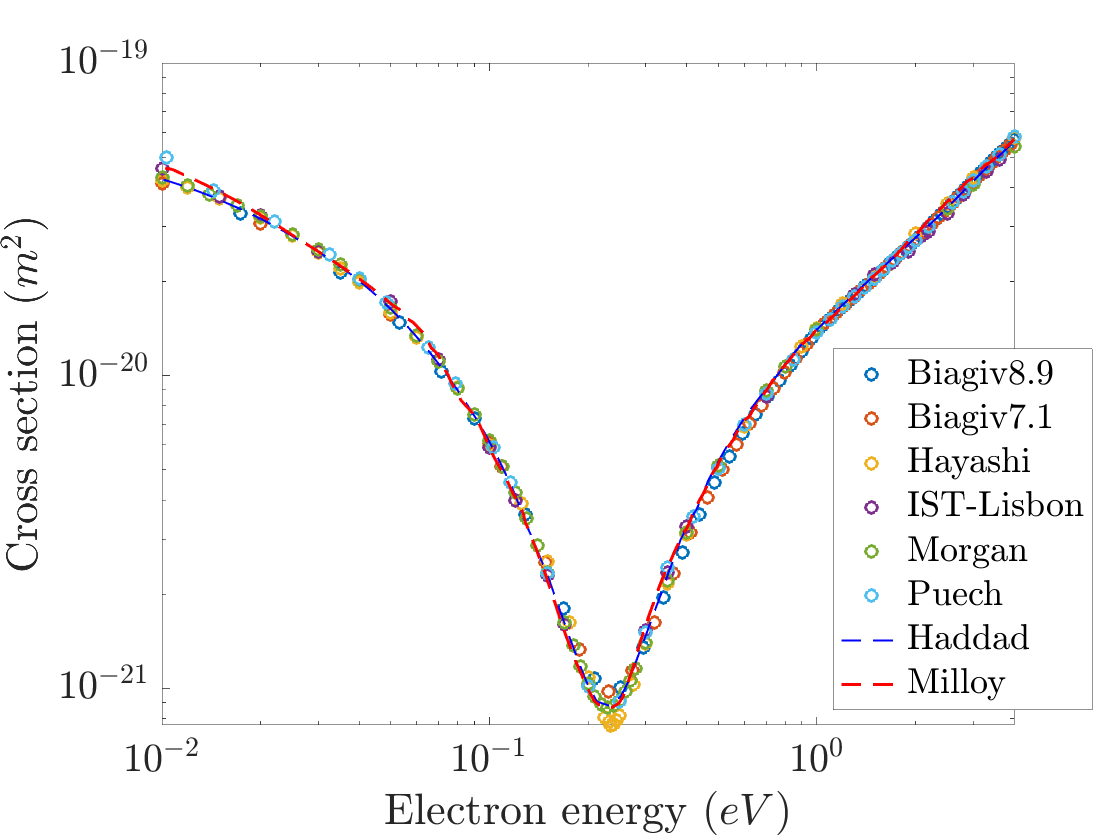
\includegraphics[width=0.5\textwidth]{./figures/milloy}
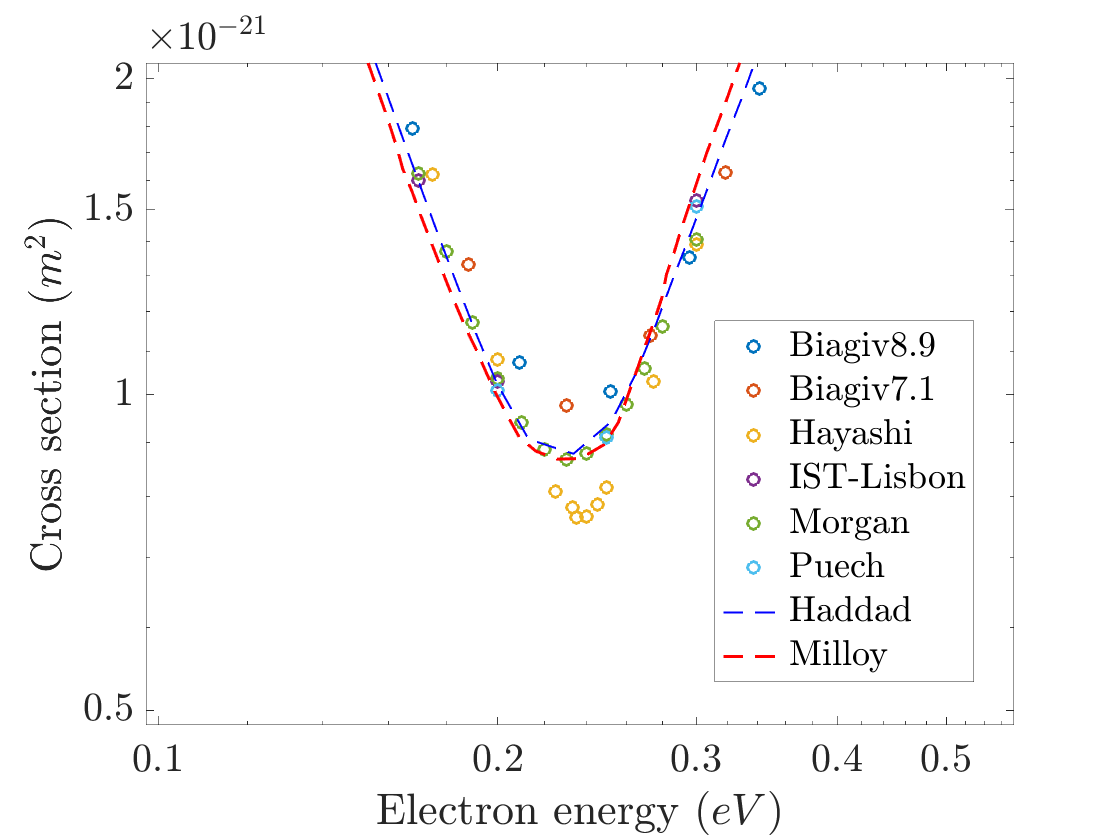
\includegraphics[width=0.5\textwidth]{./figures/milloy2}
\caption{Cross sections compared to Milloy~\cite{Milloy1977} dataset.}
\label{fig:milloy}
\end{figure}
\par
Thus the coincidence of these datasets is mainly due to overlap of the same primary source (Milloy~\cite{Milloy1977}),
and it may not imply that we have very small uncertainty around Ramsauer minimum.
Rather, Milloy~\cite{Milloy1977} specified (fortunately) the uncertainty of cross section around Ramsauer minimum is $-20\sim+12\%$ for $0.1-0.4eV$.
Milloy also reported the sensitivity of swarm parameters (especially diffusion) to the Ramsauer minimum value~\cite[Fig 1,2]{Milloy1977}.

\subsubsection{Largest variation around the peak}
The largest variations between datasets are observed for $2.5-15eV$, as shown in Figure~\ref{fig:peak}.
\begin{figure}[h]
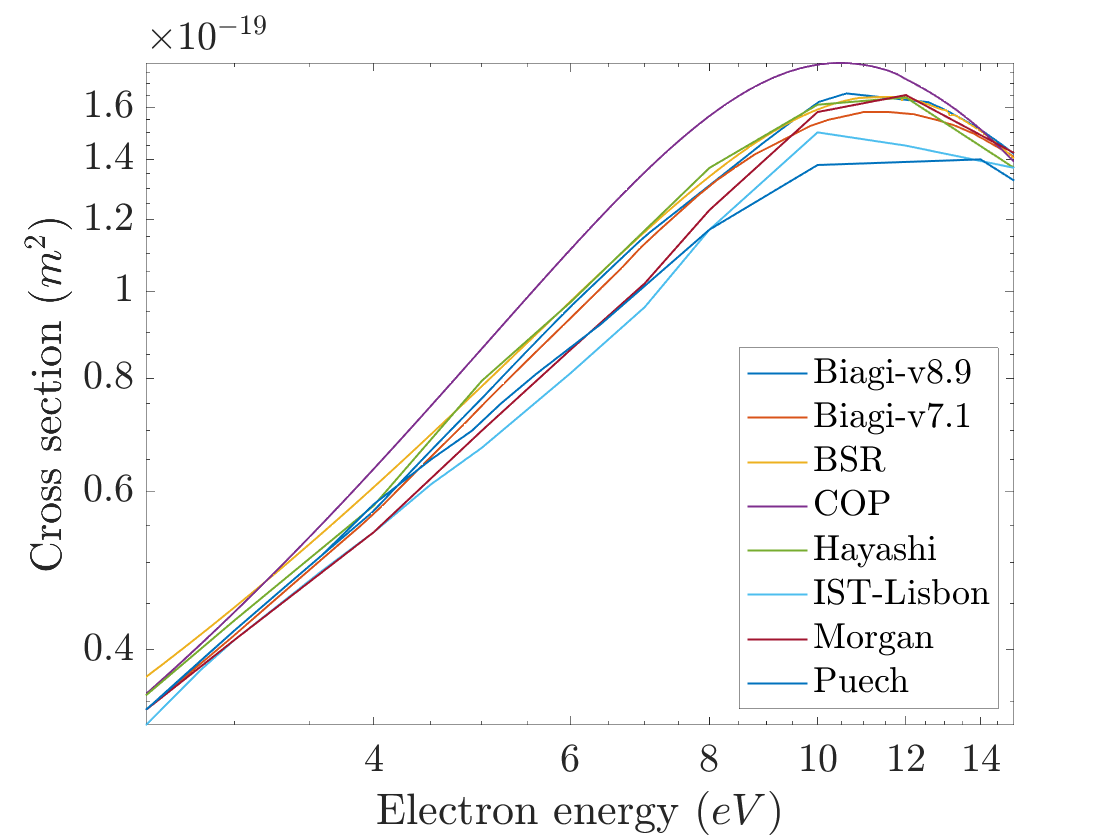
\includegraphics[width=0.6\textwidth]{./figures/peak}
\caption{Cross sections for $2.5-15eV$.}
\label{fig:peak}
\end{figure}

\subsubsection{Functional form of uncertainty at $>10eV$}
\begin{figure}[h]
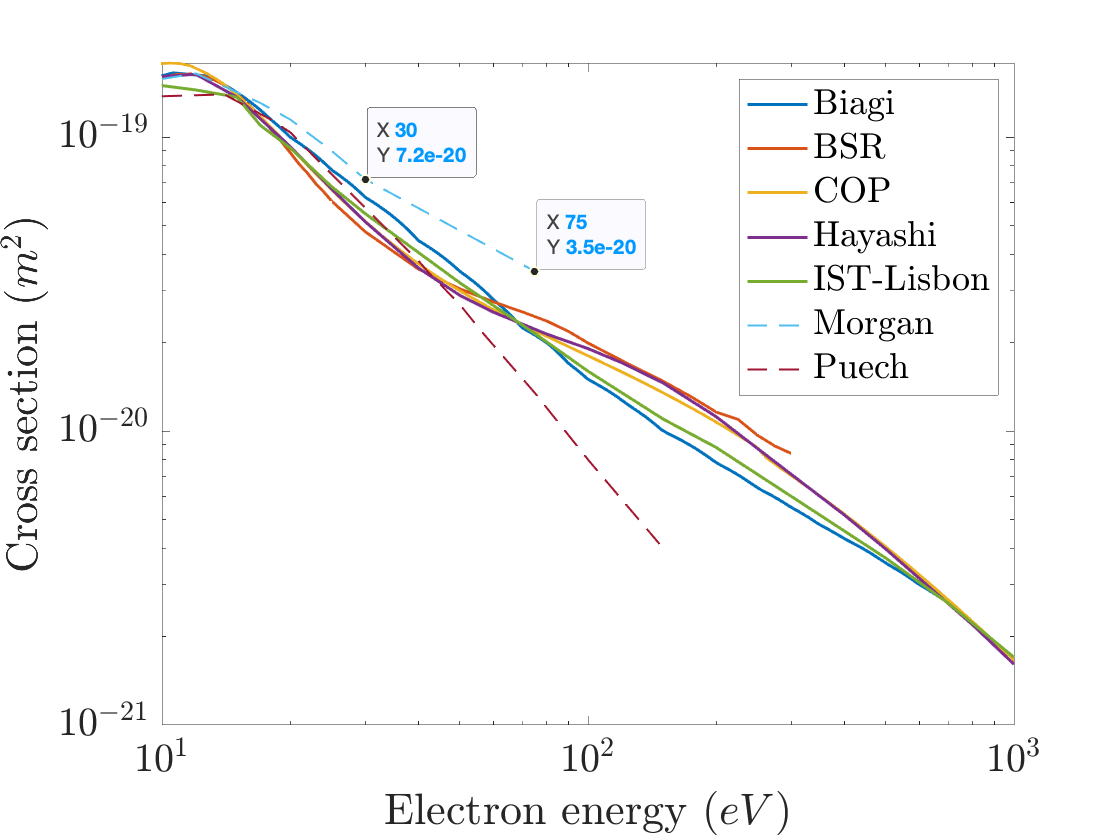
\includegraphics[width=0.6\textwidth]{./figures/elastic-biagi-bsr-cop}
\caption{Momentum transfer cross sections for $>10eV$.}
\label{fig:elastic10}
\end{figure}
Figure~\ref{fig:elastic10} shows momentum cross sections for $>10eV$.
Though may not important,
it is observed for $>10eV$ that variations between datasets are negatively correlated around $\approx70eV$, except Morgan and Puech.
The resolution of Morgan for $>30eV$ is very low, having only one value at $75eV$.
As will be shown later,
Puech dataset at this regime seems to be extrapolated from Frost and Phelps~\cite{Frost1964}.
Excluding Morgan and Puech,
the uncertainty for $>10eV$ may be modeled considering this correlation.

\subsubsection{Puech dataset at lowest/highest energy limit}
Puech~\cite{Puech1986} referenced two datasets for elastic momentum transfer:
\enquote{For elastic processes, we have used the momentum transfer cross section
given by Frost and Phelps~\cite{Frost1964} except in the range
$0.014-4eV$ where we have adopted the data of Milloy~\cite{Milloy1977}.}
Figure~\ref{fig:puech} shows Puech dataset in comparison with these two literatures.
\begin{figure}[h]
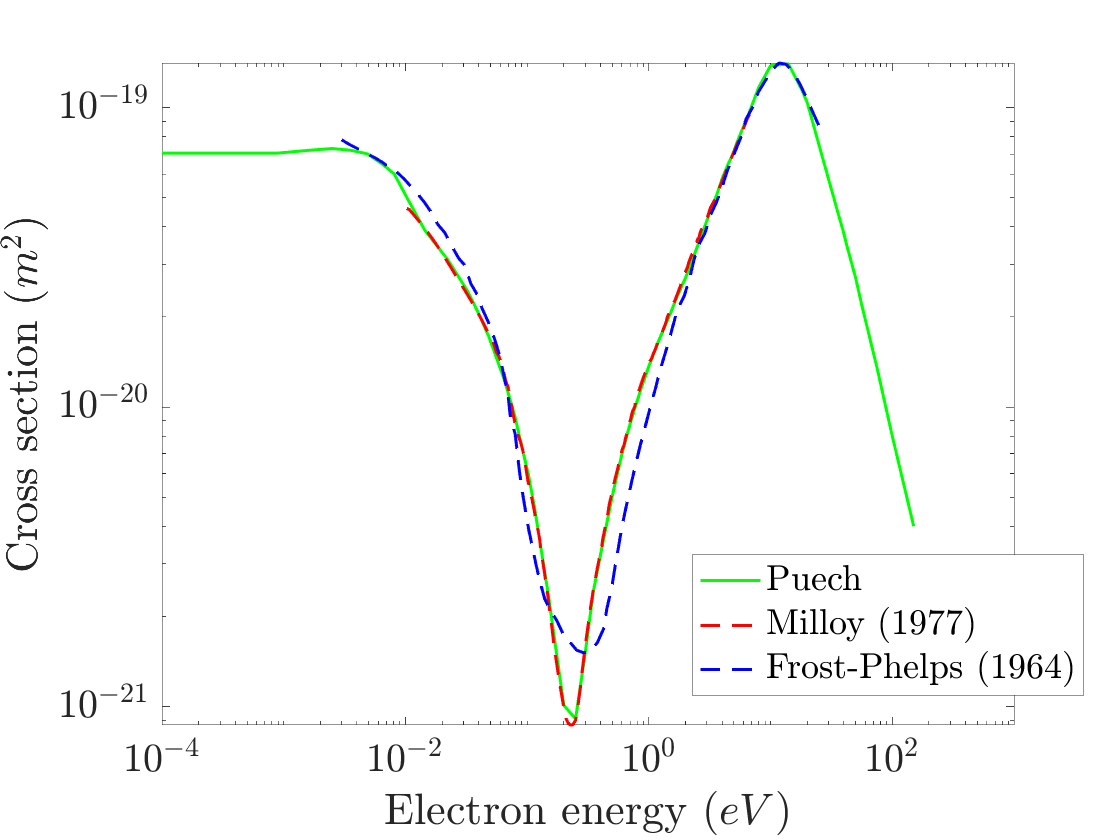
\includegraphics[width=0.6\textwidth]{./figures/puech}
\caption{Comparison of Puech~\cite{Puech1986} with Milloy~\cite{Milloy1977} and Frost and Phelps~\cite{Frost1964}.}
\label{fig:puech}
\end{figure}
Puech dataset in LXCat seems to be interpolated between these two literatures,
and extrapolated for lowest and highest energy interval not covered by them.
In this extrapolated energy regime,
functional form of Puech cross section significantly differs from others.

\subsubsection{Two elastic cross sections in BSR-500}
In LXCat, both BSR and BSR-500 are identical.
BSR-500 has two elastic cross sections (with names \textit{elastic} and \textit{momentum}),
however they refer to different quantities.
According to \cite{Zatsarinny2014}, \textit{elastic} is angle-integrated cross section,
and \textit{momentum} is momentum-transfer cross section, which is what we need.
Both match well with their respective experimental data in \cite[Fig 1,2]{Zatsarinny2014}.
The figure below compares the BSR databases with \cite{Zatsarinny2014}.
The database seems to have been adjusted after publication, and the mismatch in momentum cross section is presumably due to different combination of 500 states (78/422 versus 31/469).\\
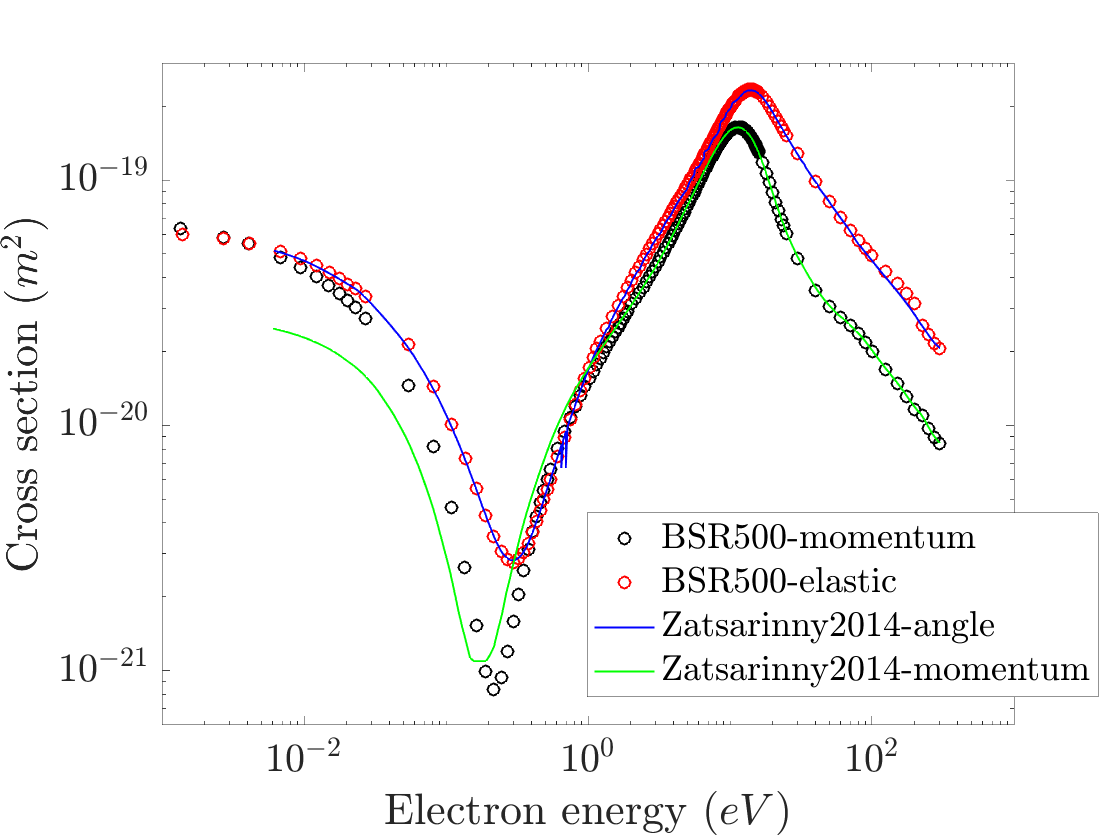
\includegraphics[width=0.6\textwidth]{./figures/bsr-elastic}

\subsubsection{Error evaluations from literatures}
\begin{figure}[h]
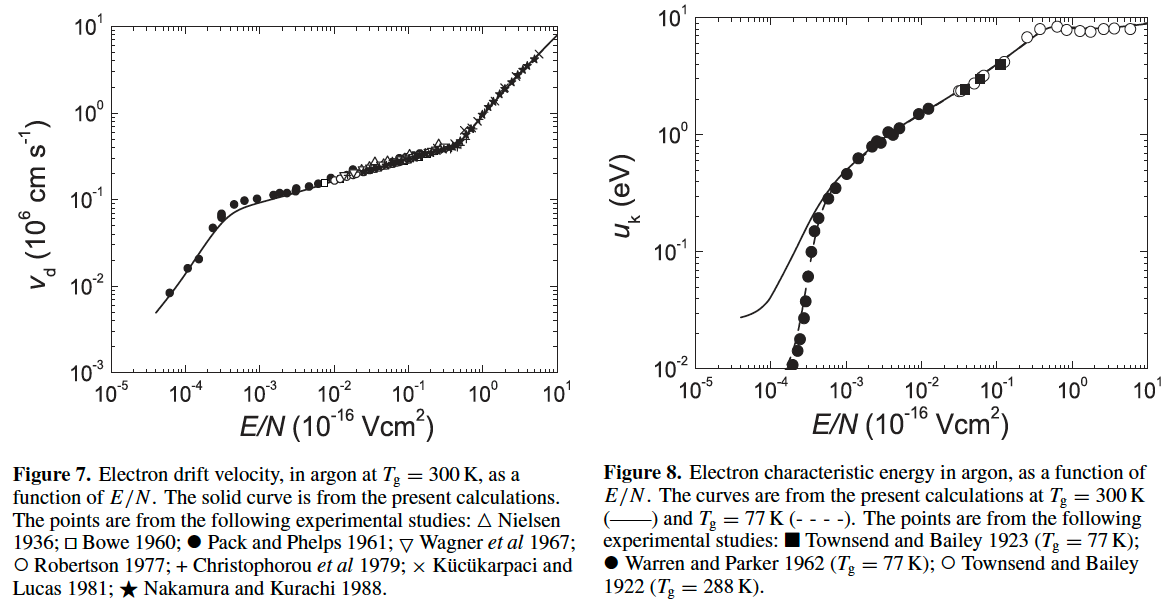
\includegraphics[width=1.0\textwidth]{./figures/yanguas2005}
\caption{IST-Lisbon: Figure 7 and 8 from \cite{Alves2005}.}
\label{fig:yanguas2005fig7-8}
\end{figure}
\begin{figure}[h]
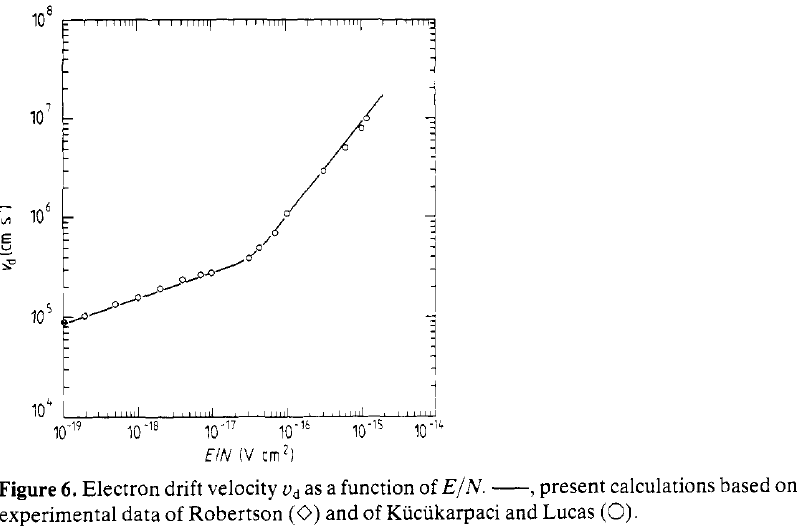
\includegraphics[width=0.6\textwidth]{./figures/puech1986fig6}
\caption{Puech: Figure 6 from \cite{Puech1986}.}
\label{fig:puech1986-fig6}
\end{figure}
\begin{figure}[h]
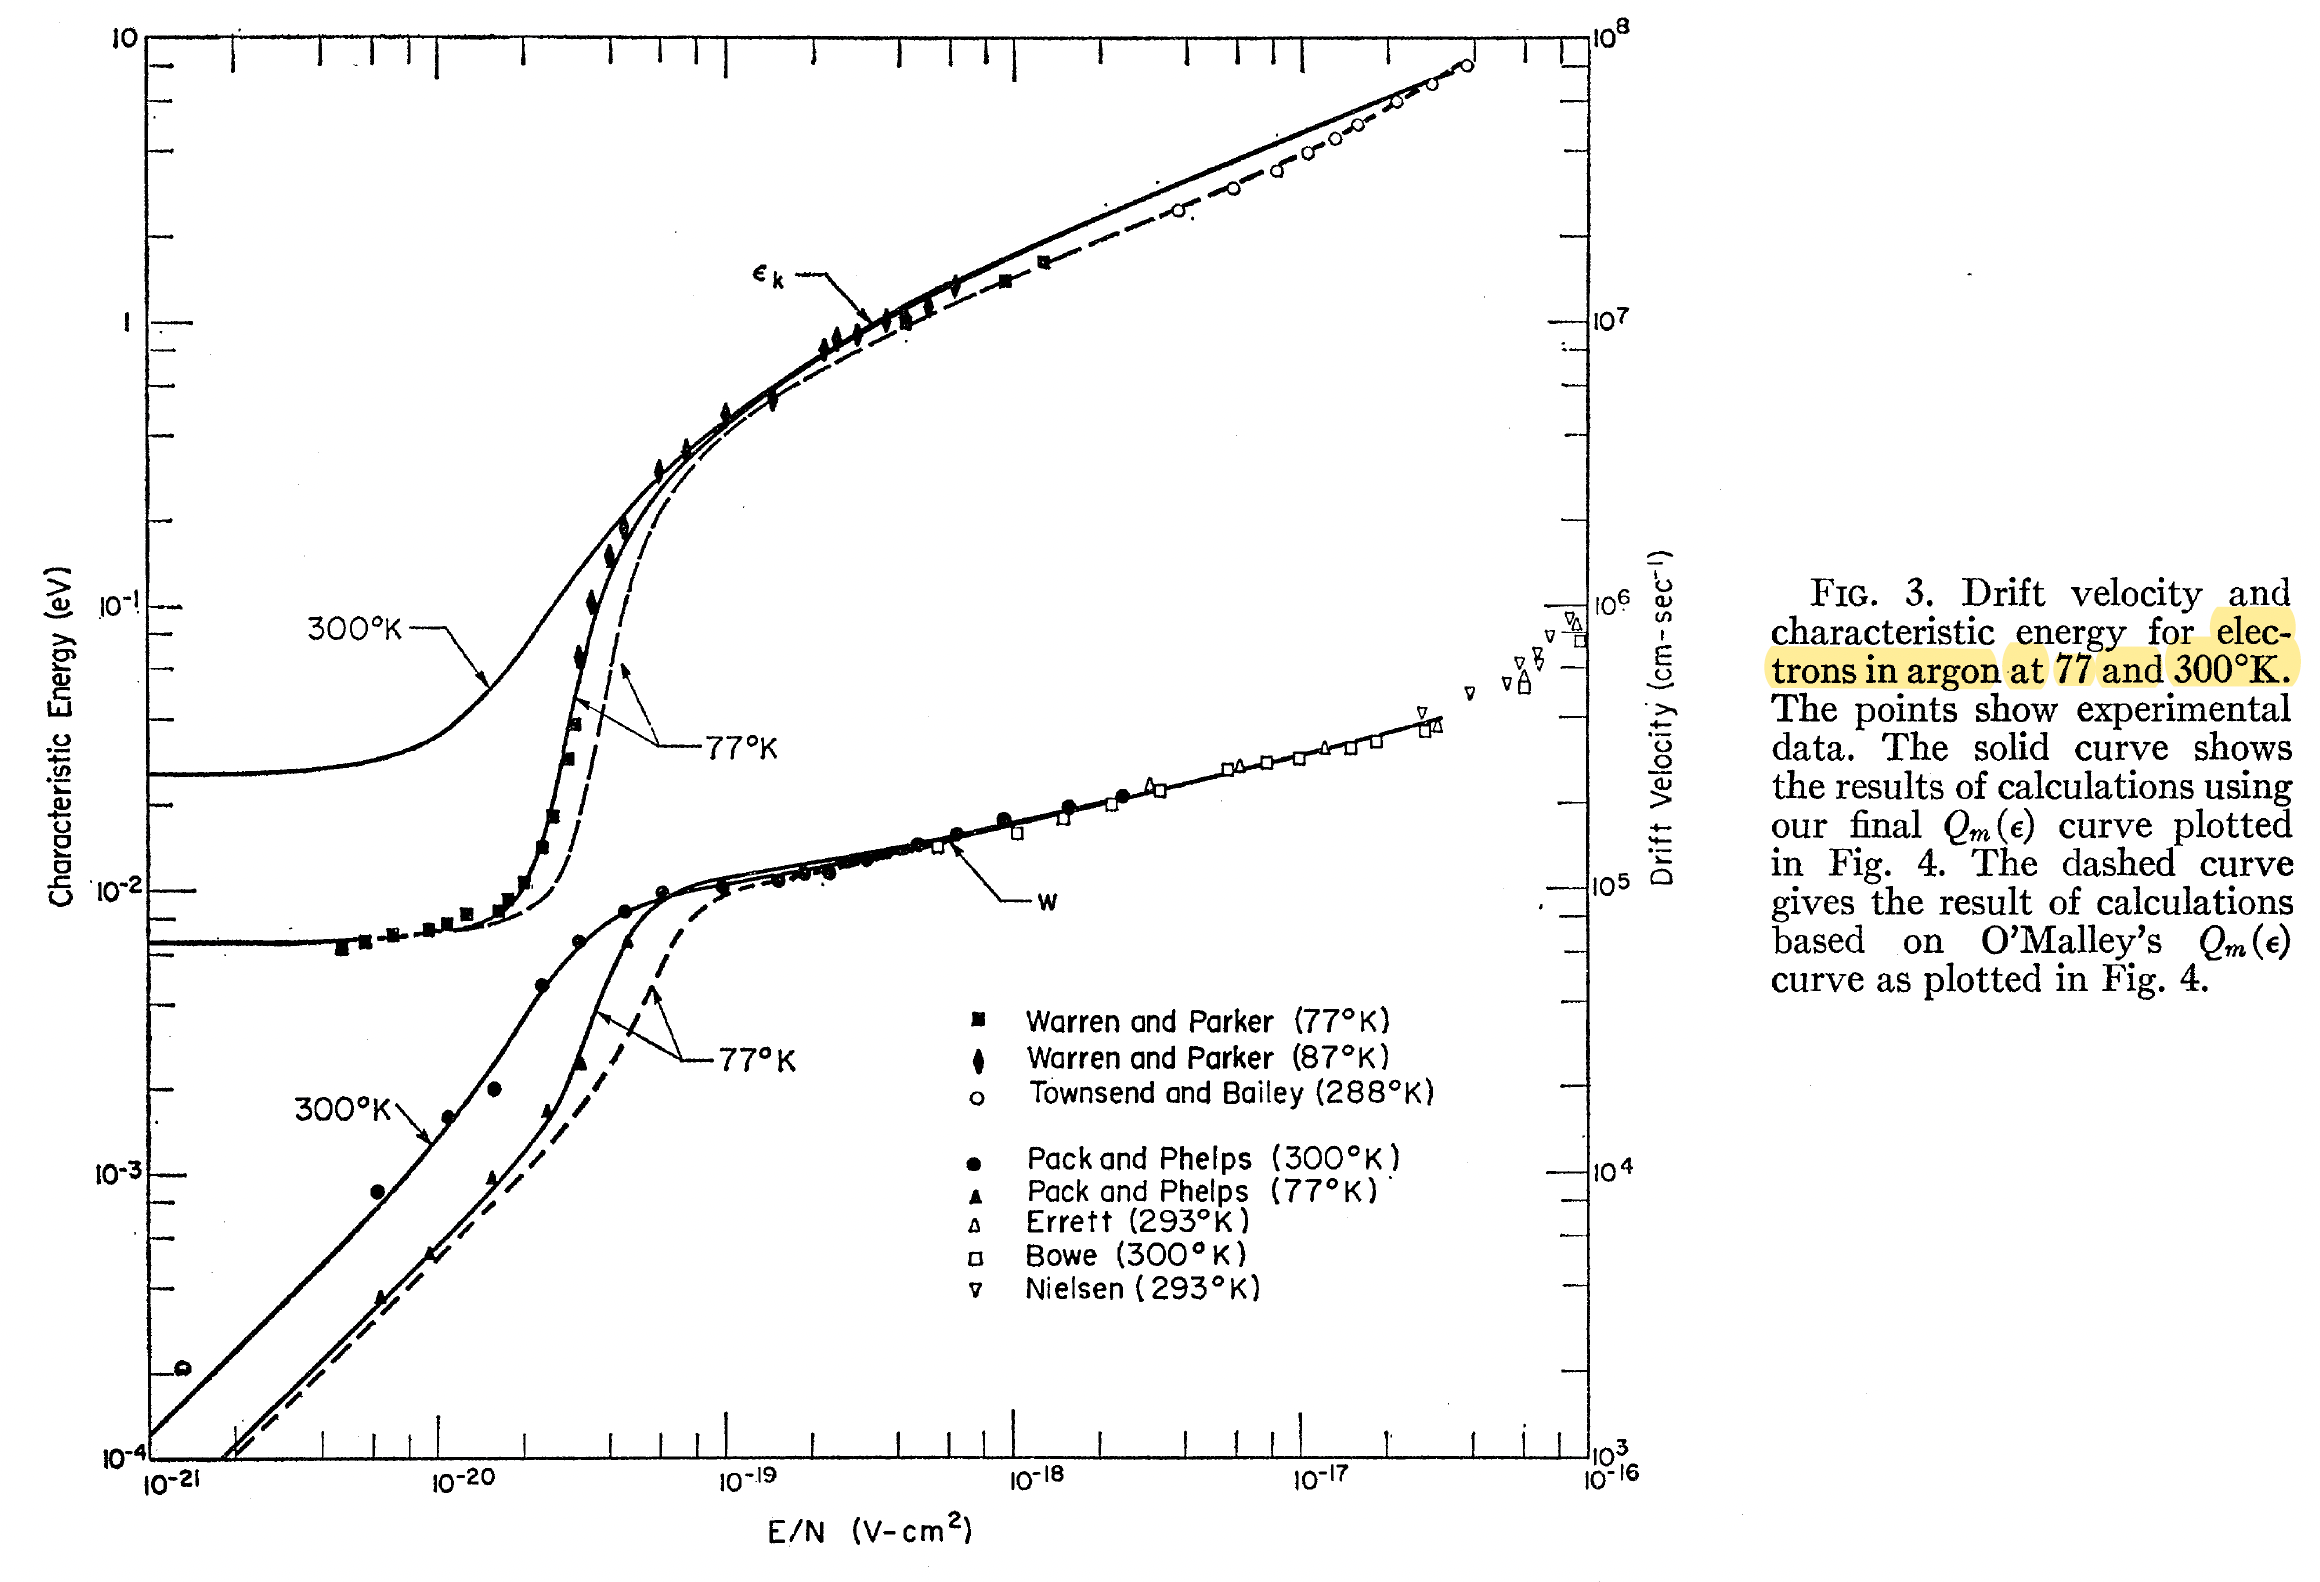
\includegraphics[width=0.6\textwidth]{./figures/frost1964-fig3}
\caption{Phelps: Figure 3 from \cite{Frost1964}. However, database is adjusted in~\cite{Tachibana1981}.}
\label{fig:frost1964-fig3}
\end{figure}
\begin{figure}[h]
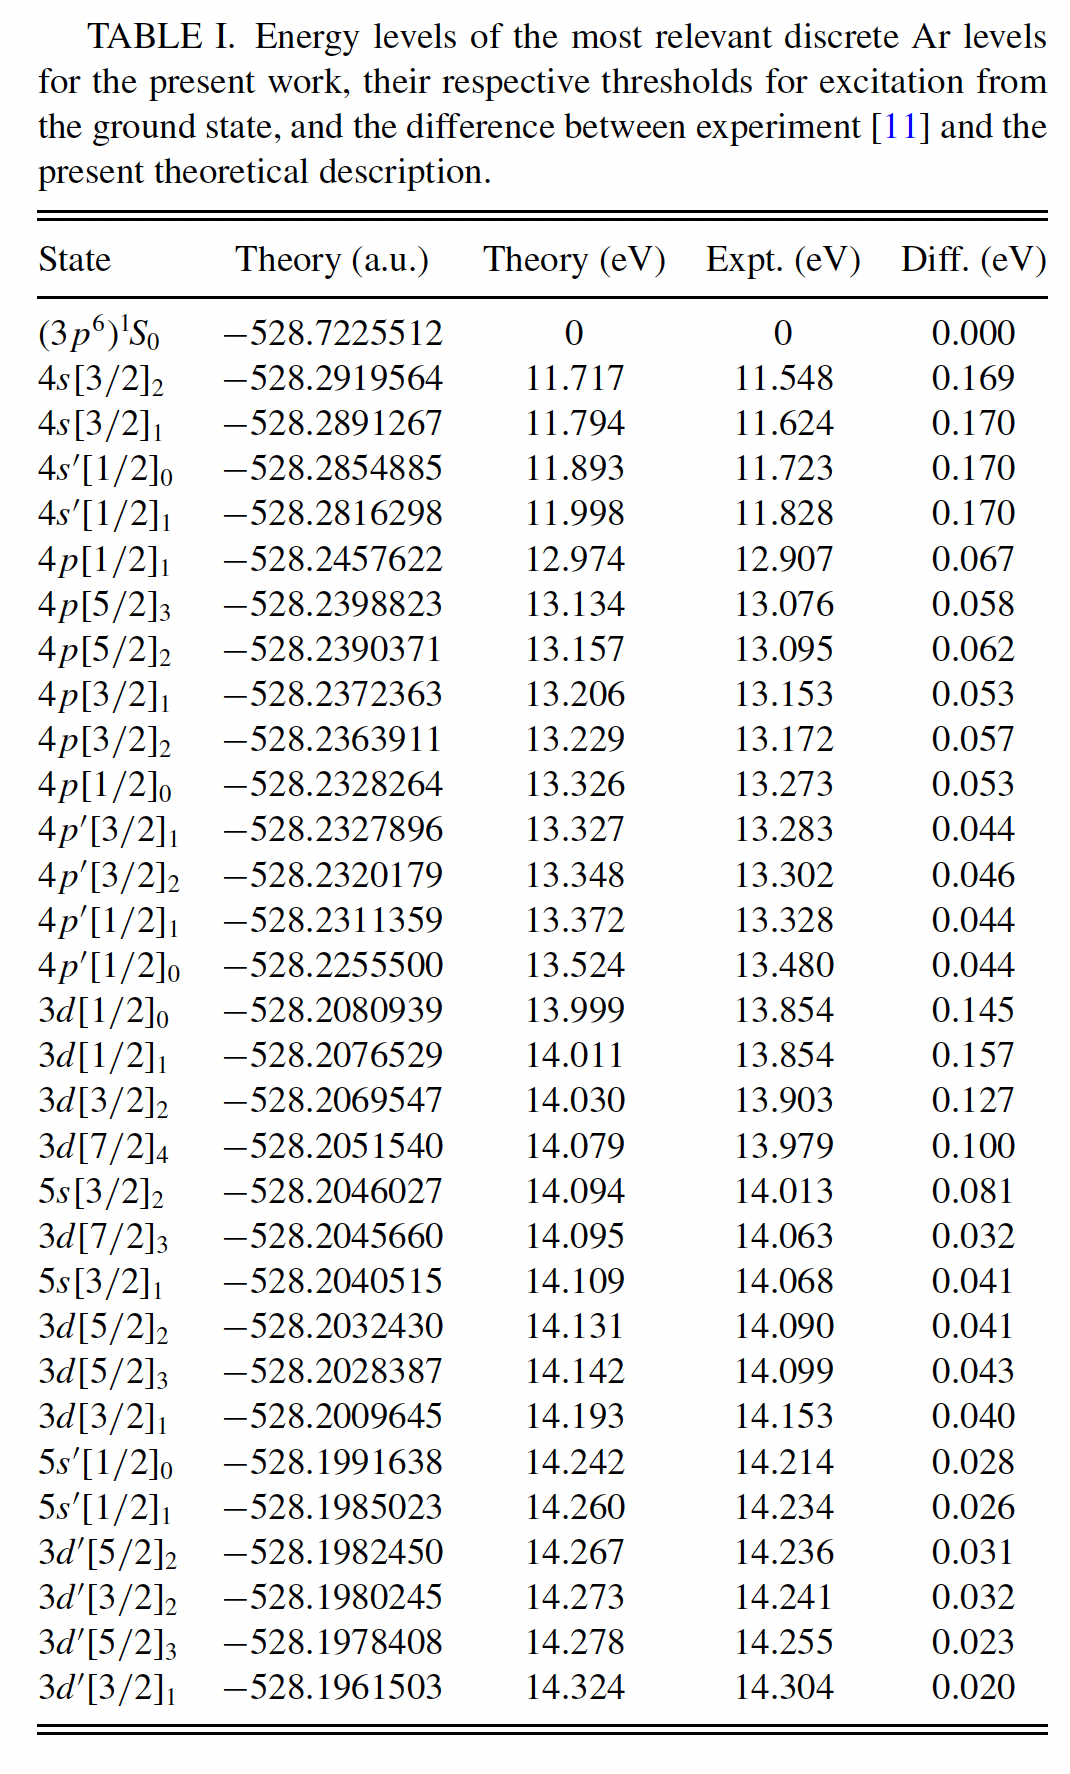
\includegraphics[width=0.4\textwidth]{./figures/zatsarinny2014-table1}
\caption{BSR: Table 1 from \cite{Zatsarinny2004}.}
\label{fig:zatsarinny2004-table1}
\end{figure}
\begin{figure}[h]
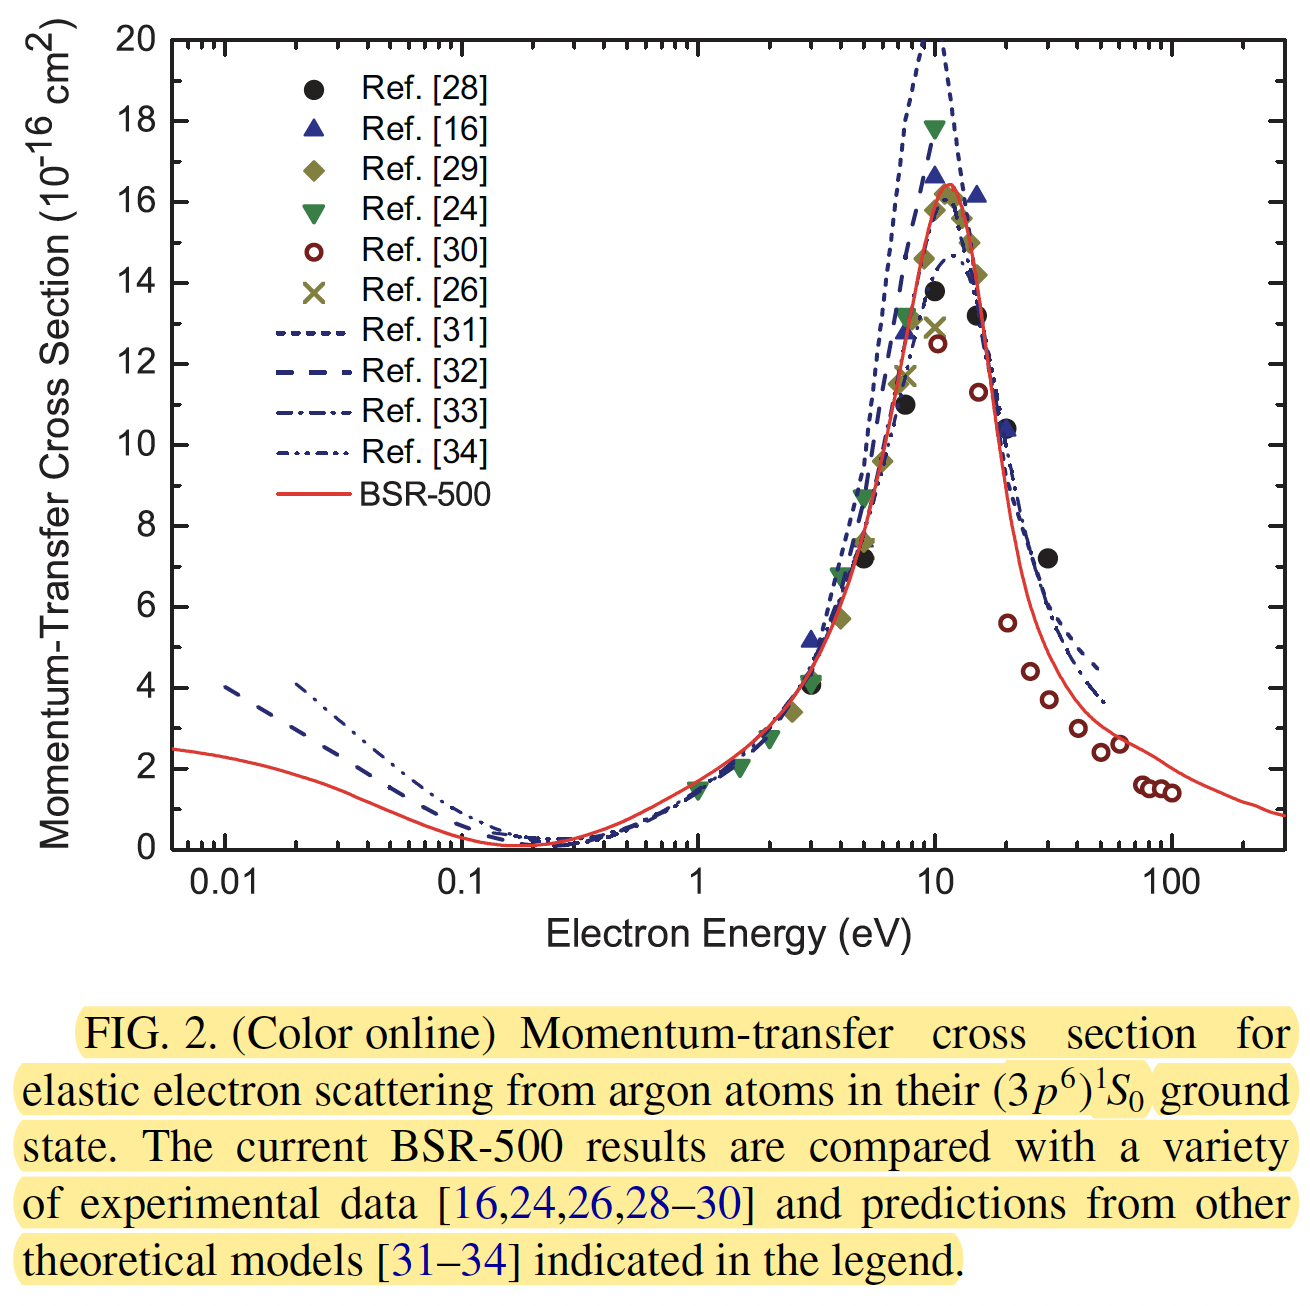
\includegraphics[width=0.6\textwidth]{./figures/zatsarinny2014-fig2}
\caption{BSR: Figure 2 from \cite{Zatsarinny2014}.}
\label{fig:zatsarinny2014-fig2}
\end{figure}
\begin{figure}[h]
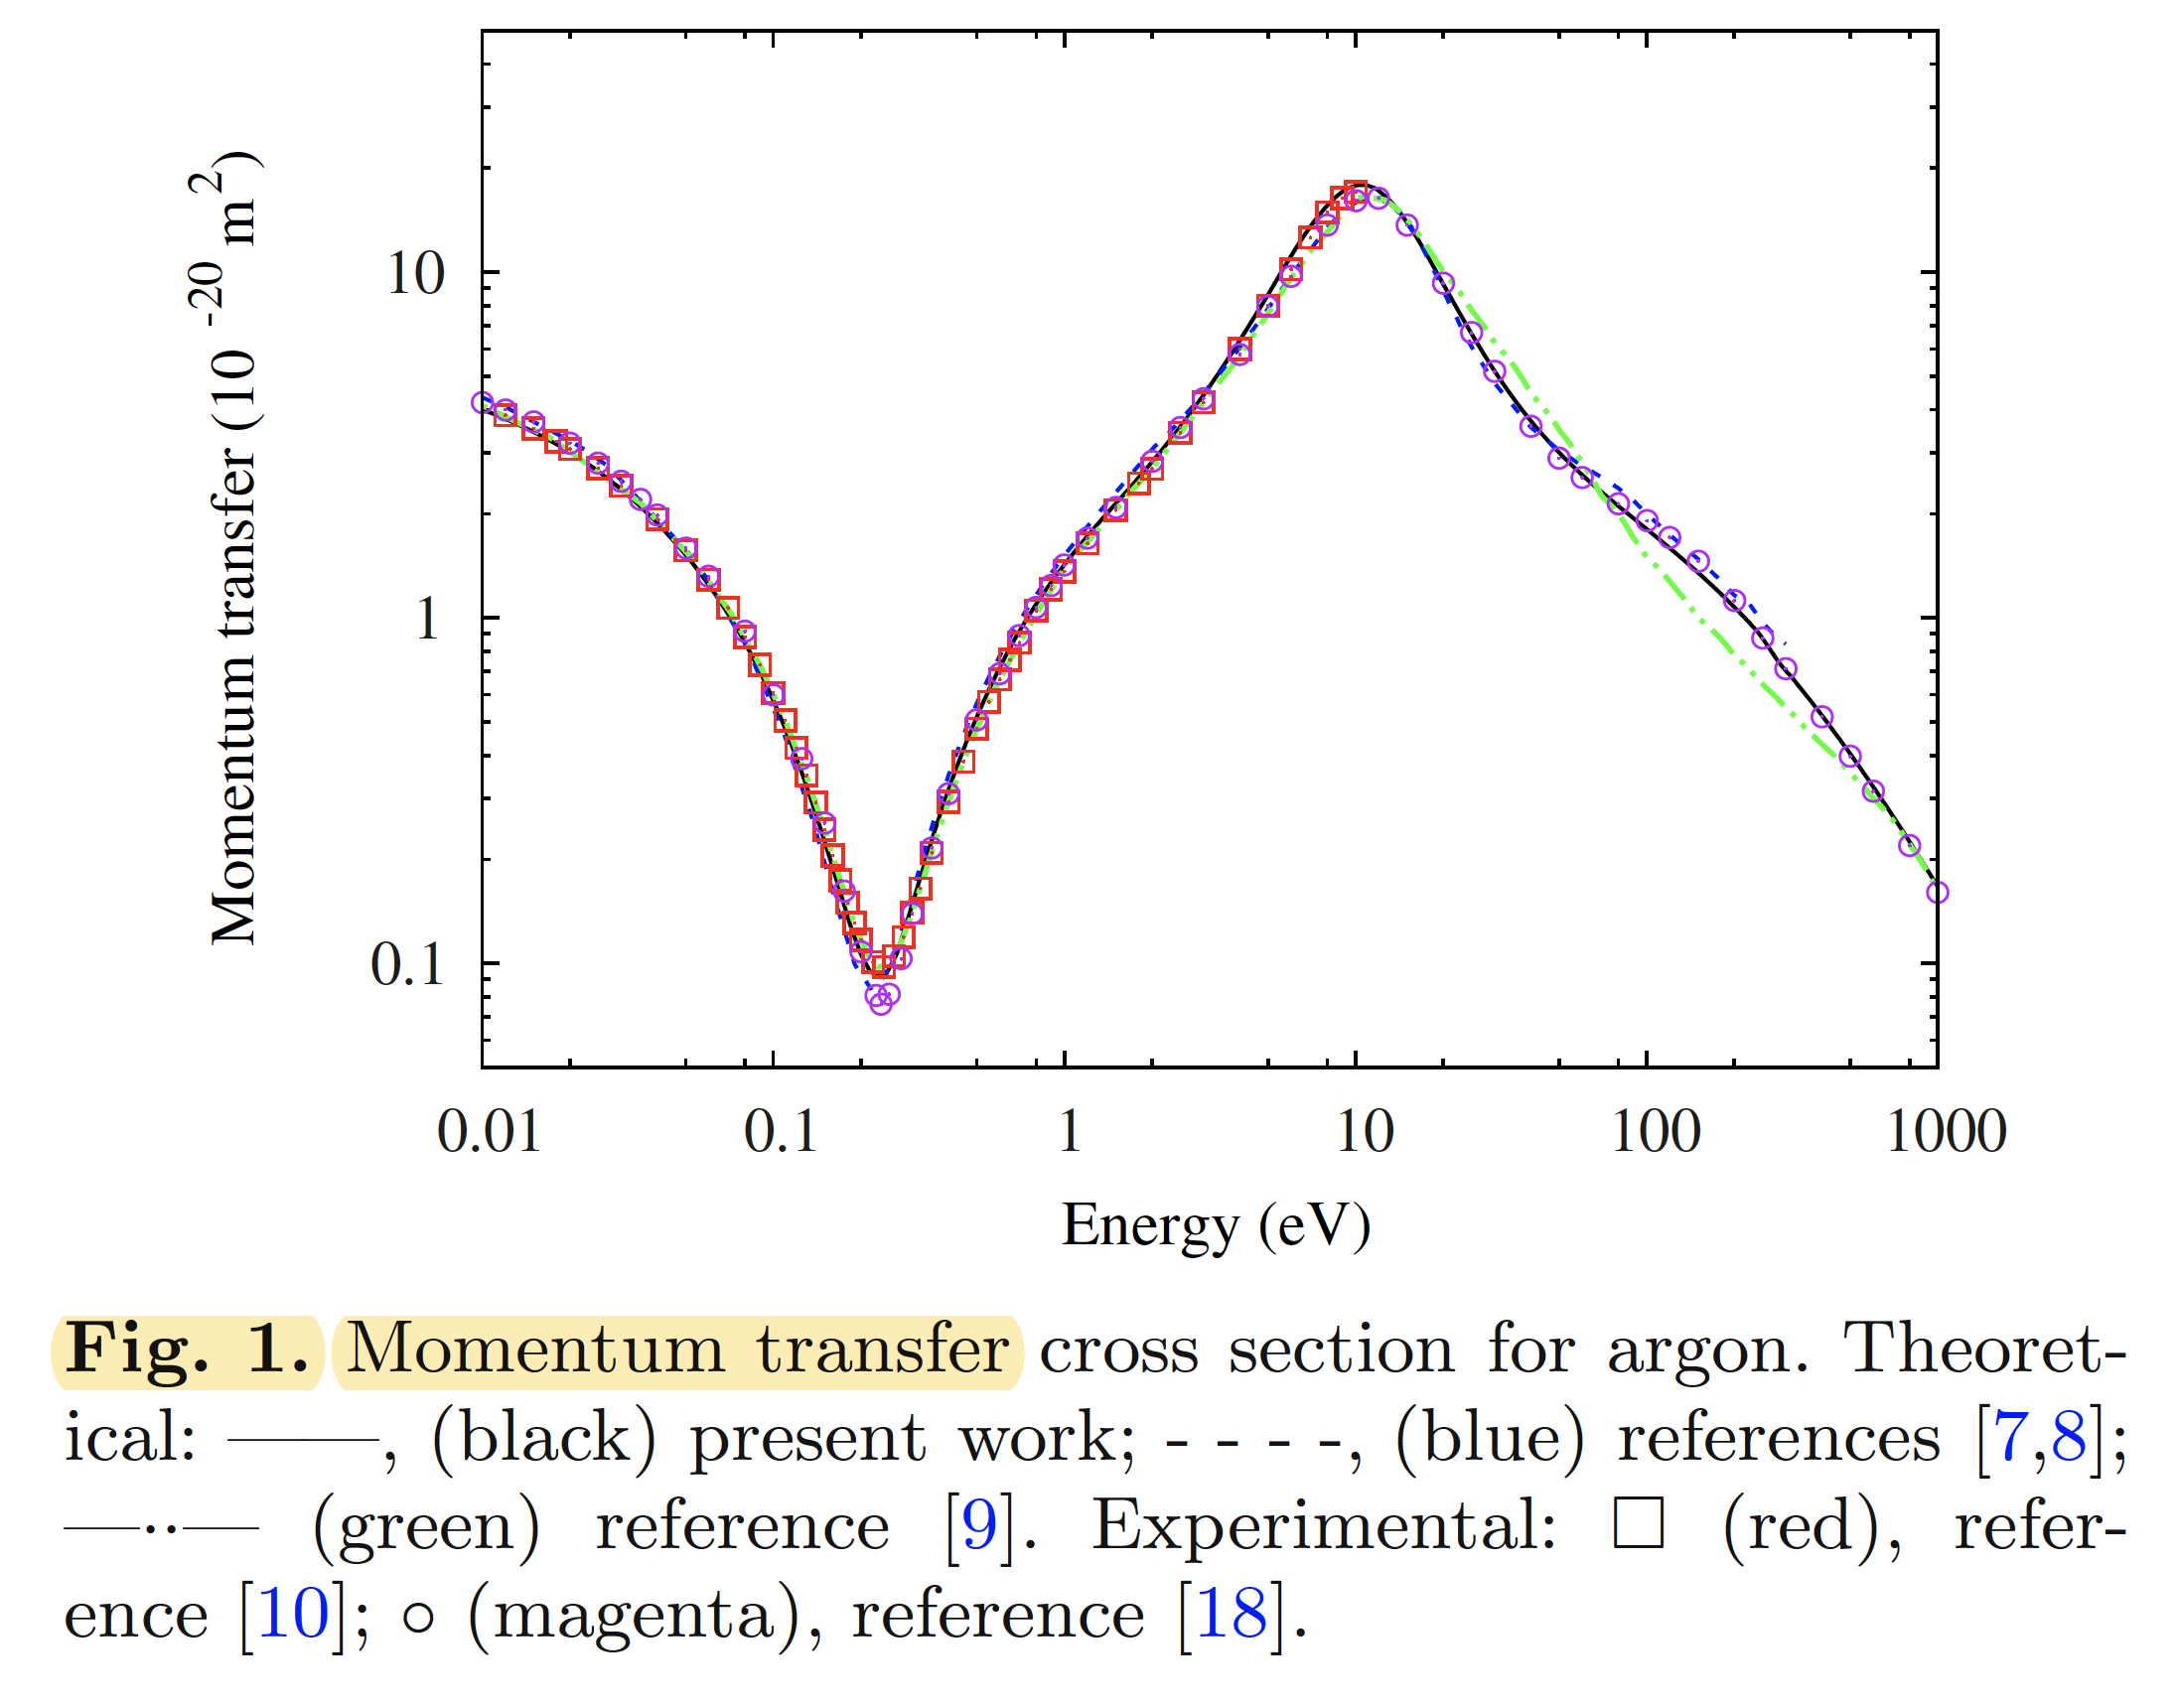
\includegraphics[width=0.6\textwidth]{./figures/mceachran2014-fig1}
\caption{COP: Figure 1 from \cite{Mceachran2014}.}
\label{fig:mceachran2014-fig1}
\end{figure}

\clearpage

\section{Total ionization cross section}
\subsection{Biagi}
\begin{itemize}
\item \cite{Pitchford2013}\\
The ionization cross section used was an average of the data from Rapp and Englander-Golden~\cite{Rapp1965} and the more recent data of Straub et al~\cite{Straub1995}.
These measurements agree within their experimental errors of 3 to 6\% which gives confidence that the ionization cross section would not be the limiting factor in the accuracy of the derived dataset.
\item \cite{Pitchford2017}\\
The consistency between these measurements~\cite{Rapp1965,Straub1995} is within typically $4\%$ and a weighted average is used in the Magboltz datasets.
\item \cite{Rapp1965}
\begin{itemize}
\item Experimental measurement
\item For a gas capable of multiple ionization, the total cross section is a charge-weighted sum of partial ionization cross sections: $\sigma_T = \sigma_1 + 2\sigma_2 + \ldots$
\item $<800 eV$ (relative cross section): within (better than) $\pm 1\%$
\item $\ge 800 eV$ (relative cross section): within $\pm 2\%$
\item Near(?) the peak (relative cross section): within $\pm 0.3\%$
\item The absolute normalization in $H_2$ (error within $\pm 4.5\%$) is used to normalize the relative cross section of $Ar$.
However, it is unclear how this should be considered in cross section uncertainty.
\end{itemize}
\item \cite{Straub1995}
\begin{itemize}
\item Specified r.m.s. uncertainty of relative/absolute cross section~\cite[Table 1]{Straub1995}: $\pm 3.5\%$
\end{itemize}
\end{itemize}

\subsection{BSR}
\begin{itemize}
\item \cite{Pitchford2013}\\
As also discussed in section 2 above, our predictions for the total ionization cross section are lower than experiment by up to about $30\%$ between threshold and the maximum of the cross section around $80eV$. Our tests so far suggest that the results are stable to better than $30\%$, and hence we can currently not explain the remaining discrepancies between the BSR results and the direct measurements of the ionization cross sections. However, assuming that at least the energy dependence of the experimental data is very reliable (more than the absolute normalization), it is likely that the BSR model needs to be further improved in this intermediate energy regime.
\item Even more pseudo-states may be required in the energy region from threshold to a few times that energy. Unfortunately, we cannot perform such calculations at the present time, simply because of the limited available computational resources.
\end{itemize}

\subsection{IST-Lisbon}
\begin{itemize}
\item \cite{Pitchford2013}\\
For direct ionization we have adopted the cross section measured by Rapp and Englander-Golden~\cite{Rapp1965}.
\end{itemize}

\subsection{Phelps}
\begin{itemize}
\item \cite{Pitchford2013}\\
It used $(\ldots)$ the ionization cross section of Smith~\cite{Smith1930}.
\item \cite{Smith1930}\\
No uncertainty is provided. 
\end{itemize}

\subsection{Puech}
\begin{itemize}
\item \cite{Puech1986}\\
For inelastic processes, we have used the set of collision cross sections previously established in paper I~\cite{Bretagne1986}.
This set of cross sections takes account of 40 individual excited levels and includes the three shells of ionization.
\item \cite{Bretagne1986}\\
Uncertainty is not provided. This is a theoretical (analytical) quantum mechanics calculation of cross section with some fitting of other literatures.
\end{itemize}

\clearpage

\section{Excitation cross section}

\begin{itemize}
\item \cite{Pitchford2013}\\
The excitation cross sections in the datasets PHELPS,
MORGAN, and BIAGI-v7.1 contain one, two, or three excitation levels, respectively, and the magnitudes of these cross sections were first estimated by theory and/or experiment and then adjusted to yield good fits to swarm parameters
\item \cite{Pitchford2013}\\
The remaining four datasets (BIAGI-v8.9, HAYASHI,
IST-LISBON and PUECH) are attempts to assemble complete sets of electron–argon scattering cross sections from beam measurements and/or theory. We will refer to these as the ‘detailed’ datasets. In all cases, some modifications or extensions of the literature values were needed to obtain consistency with swarm parameters.
\end{itemize}

Angle-integrated cross section experiment: \cite{Chutjian1981,Filipovic2000,Khakoo2003}

\subsection{Biagi}
Started from some theoretical formula $+$ some adjustment to fit swarm experiments
\begin{itemize}
\item \cite{Pitchford2013}\\
The dipole allowed states were described by BEF scaling (Kim 2001, Kim 2007) with oscillator strengths from theory and experiment which had been published up to 2010. The agreement with theory and experiment is very good (BSR~\cite{Zatsarinny2004}, Allan et al~\cite{Allan2006}, and Berkowitz~\cite{Berkowitz2002}).
\item \cite{Pitchford2013}\\
The analytical cross section fit to the BEF formula was only used above the resonance region. In the resonance region we used the cross section of Allan et al (2006) and scaled it to give a good fit to the light emission measurements of Tachibana~\cite{Tachibana1986} and the reduced ionization coefficients measured by Kruithof~\cite{Kruithof1940} for version 7.1 and by Kruithof~\cite{Kruithof1940} and Specht et al~\cite{Specht1980} for version 8.9.
\end{itemize}

\subsection{IST-Lisbon}
Direct excitation cross section up to $100eV$ were obtained~\cite{Alves2014}:
\begin{itemize}
\item \cite[Table 4]{Khakoo2003}: $4s$ metastable and resonance levels. Resonance levles are multiplied by $0.5$. Error specified.\\
LXCat data seems to be interpolated from the experimental values above, having higher energy resolution.
It is not clear why they multiplied the factor of $0.5$.
\item \cite[Figure 8]{Chilton1998}: $4p$ levels. Error bar plotted.
\item \cite{Pitchford2013}\\
The previous direct excitation cross sections were extended from 100 eV to 1 keV, by using analytical asymptotic expressions ``similar to'' those proposed by Bretagne et al (1986) and Bretagne et al (1982) (based on the time- dependent perturbation theory in conjunction with the first Born approximation).
\item \cite{Pitchford2013}\\
The IST-LISBON dataset is based mainly on measurements. Only one adjustment was made in order to improve the agreement with measured swarm parameters--- a scale factor of 0.5 was applied to the measurements of Khakoo et al (2004)~\cite{Khakoo2003} for the resonance levels
\end{itemize}

\subsection{BSR}
\begin{itemize}
\item \cite{Pitchford2013}\\
The excitation results, especially for incident projectile energies above the ionization threshold and for weak, optically forbidden transitions, are very sensitive to details of the theoretical model. Models that only include discrete states, such as the 31-state calculation (Zatsarinny and Bartschat 2004), are expected to generally overestimate the true excitation cross sections.
($\ldots$) As discussed in section 2 of this paper, the BSR-500 cross sections are even somewhat lower than many experimental data, while the BSR-31 cross sections were certainly too large.
\end{itemize}

\subsection{Puech}
\begin{itemize}
\item \cite{Puech1986}\\
For inelastic processes, we have used the set of collision cross sections previously established in paper I~\cite{Bretagne1986}.
This set of cross sections takes account of 40 individual excited levels and includes the three shells of ionization.
\item \cite{Bretagne1986}\\
Uncertainty is not provided. This is a theoretical (analytical) quantum mechanics calculation of cross section with some fitting of other literatures.
For a forbidden transition to state $j$ (metastables?),
\begin{equation}
\sigma_j = \frac{8\pi a_0^2 R}{mc^2\beta^2}b_jB_j,
\end{equation}
and for an allowed transition (resonance?)
\begin{equation}
\sigma_j = \frac{8\pi a_0^2 R^2}{mc^2\beta^2}\frac{F_{0j}}{W_j}\left[ \ln\left(\frac{\beta^2}{1-\beta^2}\frac{2mc^2}{R}C_j\right) - \beta^2 \right]B_j,
\end{equation}
where $B_j$ is an empirical low-energy modifier,
\begin{equation}
B_j = \frac{ [ 1 - (2W_j/mc^2\beta^2)^{\alpha_j} ]^{\beta_j} }{(mc^2\beta^2)^{\gamma_j}}.
\end{equation}
\item \cite{Bretagne1986}\\
Figure 1 and 2 show three lowest excitation levels, compared with experimental measurements~\cite{Chutjian1981}. Table 1 and 2 show the parameter values for theoretical formula they used.
\end{itemize}

\appendix
\section{Quotes from literatures --- Argon momentum transfer}

\subsubsection{Biagi}
A comment from Biagi in \cite{Pitchford2013}:
\blockquote{
The measurements at the Ion Diffusion Unit at Australian
National University (see for example, \cite{Robertson1977})
showed that the sensitivity of the measurements drift
velocity to impurities can be large. For drift velocities,
I propose that the best choice is to exclude data before
the late 1960s as the measurements were done with
up to $20ppm$ of impurities in the gases. The drift
velocity measurements are the best test of cross sections
measurements since they are the most accurate. Thus, we
limit the comparisons to measurements to those with $\pm1\%$
statistical and systematic errors or better where possible.
}
Comments in \cite{Pitchford2013} related to Biagi:
\blockquote{
The cross section sets for argon in both of these databases
were derived from fitting to accurate drift velocity and
diffusion measurements using double shutter drift tubes with
variable drift distances (Nakamura~\cite{Nakamura1988}).
($\ldots$)
At higher values of E/N, the drift velocity measured by
Nakamura~\cite{Nakamura1988} is taken as the most accurate
and both cross section sets fit well to these measurements with
less than $1\%$ deviations on average.
($\ldots$)
In the
original derivation of the set 7.1 we used compatible values
of the $s$-state cross sections to those used by~\cite{Nakamura1988} and as a result we obtained and used a similar elastic
momentum-transfer cross section above $1.0 eV$.\\
It became apparent after the publications of \cite{Allan2006}
that the cross sections for the s-states close to threshold
were much higher than were used in the version 7.1 dataset.
This fact and the need to model more accurately the light
emission from excimers (\cite{Oliveira2011}) and the Penning
transfers in argon gas mixtures (\cite{Sahin2010}) led to the
development of the cross section set 8.9 with a more accurate
description of the level structure. The momentum-transfer
cross section at the peak in version 8.9 is slightly higher than
in 7.1 in order to compensate for the different excitation cross
section.
}
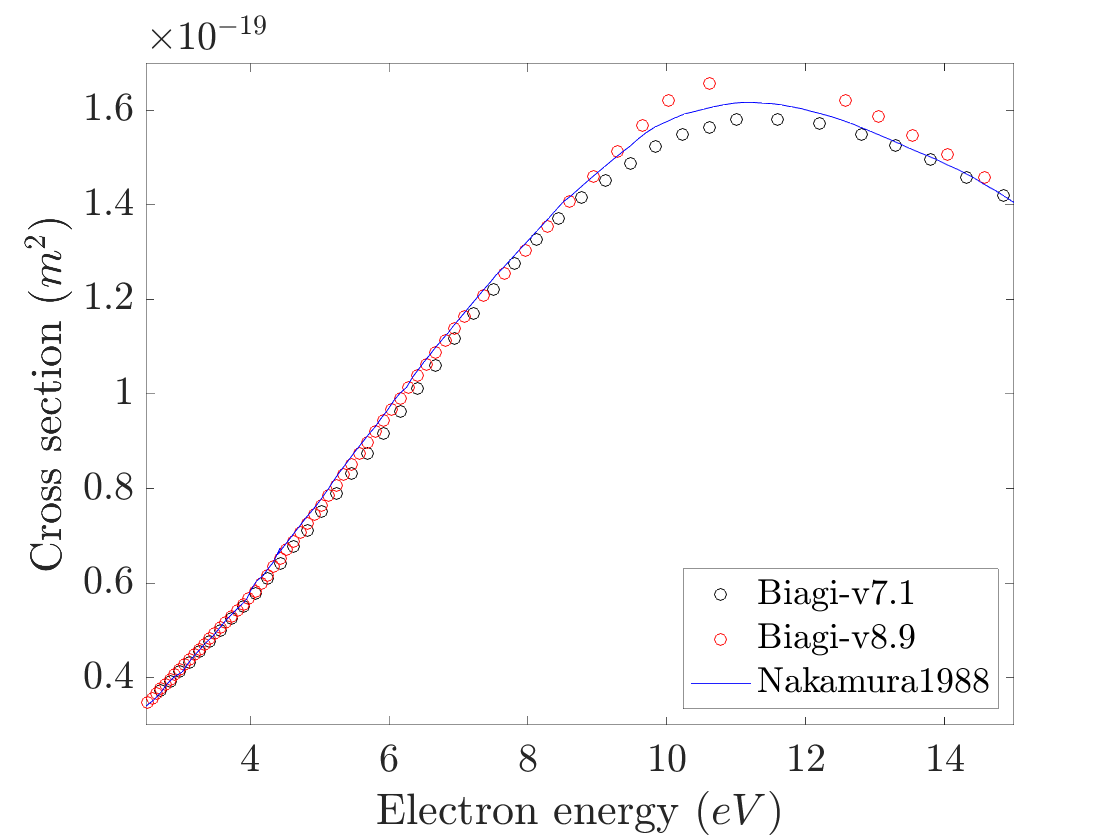
\includegraphics[width=0.5\textwidth]{./figures/collision_dependency}

Followings are the details of Nakamura~\cite{Nakamura1988}.
\begin{itemize}
\item Experiment: double shutter drift tube~\cite{Nakamura1987}
\item Measurement: drift velocity ($W$) and longitudinal diffusion coefficient (times number density, $ND_L$) of electron
\item Measurement error
\begin{itemize}
\item Drift velocity: maximum possible error $2\%$, typical standard deviation less than $1\%$
\item Longitudinal diffusion coeff. (presumably $ND_L$): maximum possible error $10\%$, typical error not specified ("larger scatter")
\end{itemize}
\item Numerically solved the equation (2-4) in \cite{Lowke1969}. Used a backward integration procedure using the Runge--Kutta method. See \cite{Parker1969,Lowke1969,Frost1962}\\
%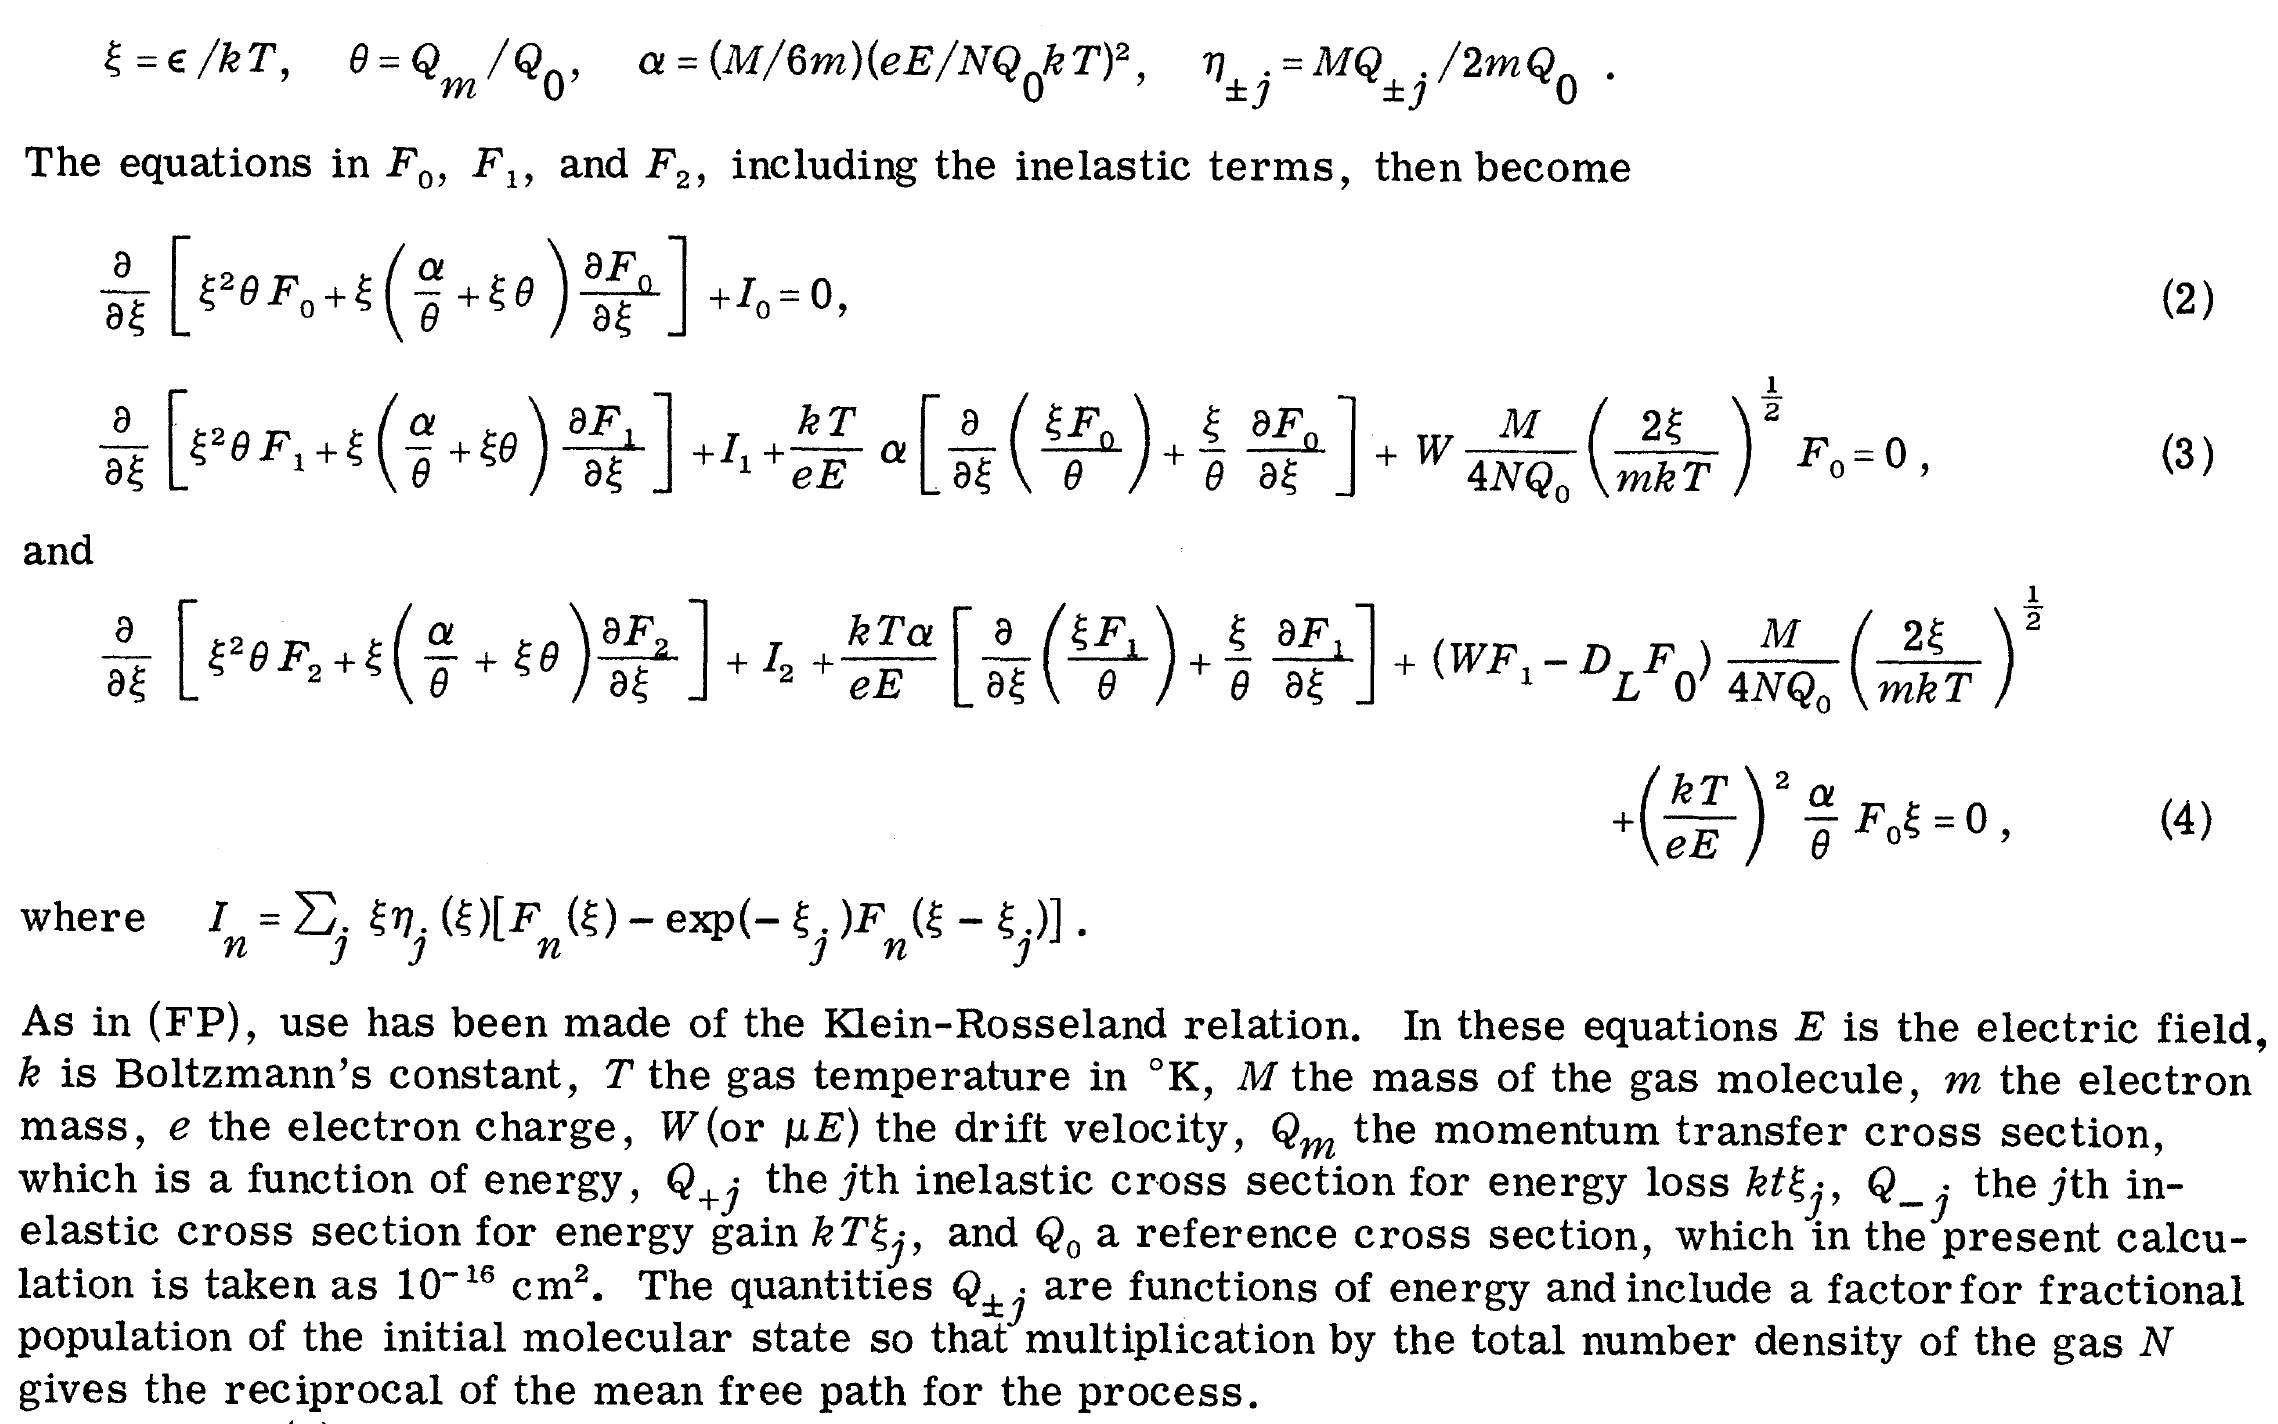
\includegraphics[width=1.0\textwidth]{./figures/lowke1969-eq234}
\item The analysis above focused on the range of electron energy $2.5eV$ to $15eV$,
and other sets of collision cross sections are combined:
\begin{itemize}
\item $\le2.5eV$: \cite{Milloy1977}
\item $\ge15eV$: \cite{Fon1983}
\item Excitation cross section: \cite{Ferreira1983}
\item Ionization cross section: \cite{Rapp1965}
\end{itemize}
\item Resulting drift/diffusion property from the ``derived" cross section\\
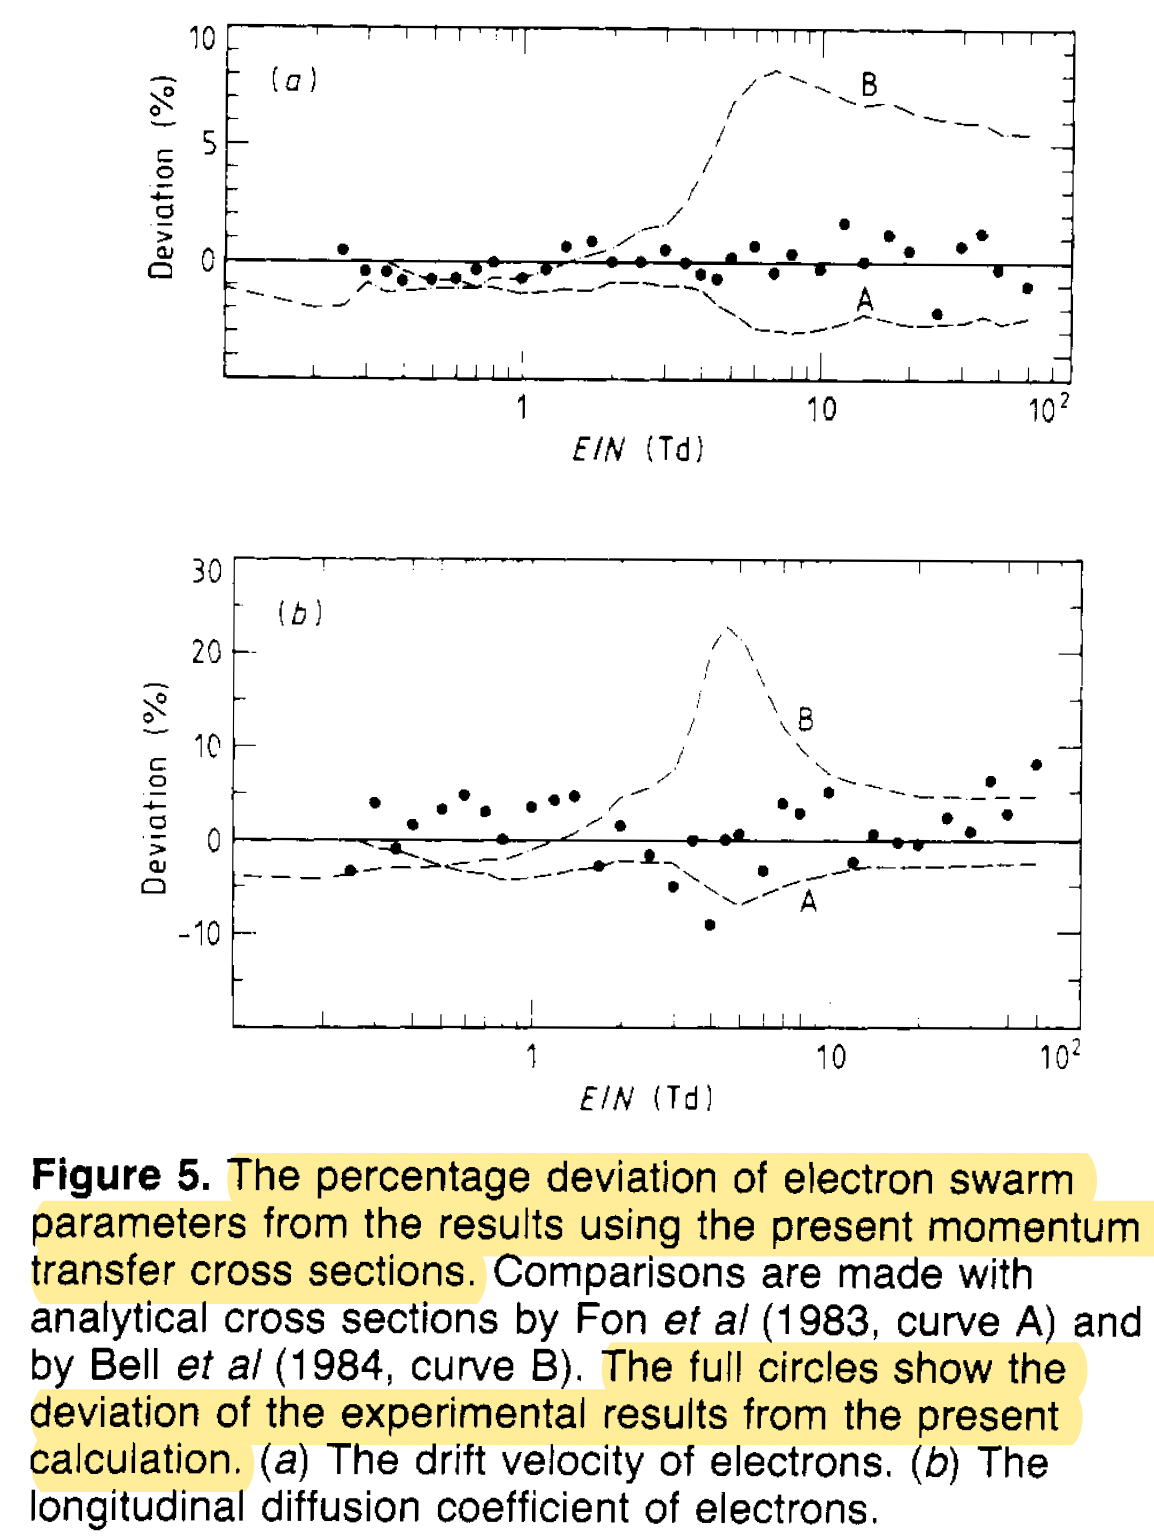
\includegraphics[width=0.6\textwidth]{./figures/nakamura1988-fig5}
\end{itemize}

\subsubsection{BSR-500}

Comments from \cite{Zatsarinny2014}:
\blockquote{
Over the years,
several experiments have been carried out and many other
calculations were performed for comparison. Many of the
numerical models were designed to treat elastic scattering
and hence it is not surprising that the overall agreement
between experiment and theory is generally satisfactory (see,
for example, [1] for detailed comparisons and also Fig. 2
below). It is however worth noting that our BSR approach can
handle the entire energy range with a single approach, which
is also used to treat the excitation and ionization processes
discussed in the following subsections.
}

Comments in \cite{Pitchford2013} related to BSR:
\blockquote{
We believe the elastic and momentum-transfer cross
sections to be accurate at the level of a few per cent. This
assessment is supported by the excellent agreement seen
in this paper between modeling predictions using these
cross sections and the corresponding experimental data.
}

Pseudo states approximation in BSR~\cite{Zatsarinny2013}:
\blockquote{
The use of `pseudo-orbitals' and `pseudo-states' constructed
with at least one of these orbitals being in a dominant
configuration has a long history in atomic structure and
collision calculations. Generally speaking, their role is
twofold: they can be used to account for (i) the term
dependence of the physical orbitals and (ii) the coupling to
the ionization continuum.
}

\subsubsection{Hayashi}
\begin{itemize}
\item Reference: \cite{Pitchford2013,Pitchford2017,Hayashi2003}
\item Compilation of 1960 references
\item ($\ldots$) The cross sections were determined from available data from electron beam and
electron swarm experiments via the Boltzmann equation and
the Monte Carlo simulation method. The beam data were given
highest priority, and theoretical values of cross sections were
sometimes used.
\item Error magnitude is not provided
\end{itemize}

\subsubsection{IST-Lisbon}
\begin{itemize}
\item LXCat reference: \cite{Pitchford2013,Pitchford2017,Alves2014}
\item \cite{Pitchford2017}\\
For each gas the database presents a complete set of cross sections,
validated against measured swarm parameters by solving
the two-term homogeneous electron Boltzmann equation.
In most cases, predictions are in agreement with
measurements within $1\sim20\%$, for reduced electric fields
$E/N = 10^{-4} \sim 500 Td$.
\item \cite{Pitchford2013}\\
The compilation and adjustment of our complete set of
electron-neutral scattering cross sections from ground-state
argon is reported in the following work: (Yanguas-Gil~\cite{Alves2005}).
This paper presents detailed comparisons between
our final set of cross sections and the ones proposed by other authors.
The elastic momentum-transfer cross section was
obtained from Phelps ftp://jila.colorado.edu/collision-data/
electronneutral/electron.txt (Yamabe~\cite{Yamabe1983}).
\item \cite{Alves2014}\\
In general, our cross sections yield predictions for the electron transport parameters and rate coefficients,
calculated with a two-term Boltzmann solver, which agree within less than $20\%$ with measurements,
for reduced electric fields $E/N=10^{-4}\sim 500Td$.
\item \cite{Alves2014}\\
$\ldots$ The compilation and adjustment of the complete set of electron–neutral scattering cross sections from
ground-state argon is reported in~\cite{Alves2005}. The set includes 39 cross sections (elastic momentum-transfer,
37 excitations and ionization) up to 1 keV.\\
$\ldots$ The elastic momentum-transfer cross section was obtained from~\cite{Yamabe1983}.
\item \cite{Alves2005} --- The updated set is
validated by comparing calculated swarm parameters and rate coefficients
(obtained by solving the two-term approximation electron Boltzmann
equation) with available experimental data.\\
$\ldots$ This work follows the recommendations of Phelps and
co-workers, adopting a total momentum transfer cross section
$\sigma_m$ that includes the elastic contribution $\sigma_{m,el}$ proposed by
\cite{Phelps1997} and by~\cite{Yamabe1983}, and the
total inelastic contribution calculated (for coherency) from the
cross section set adopted here, $\sigma_m = \sigma_{m,el} + \sigma_{t,exc} + \sigma_{ion}$.\\
$\ldots$ Simulation results for the electron drift velocity and
characteristic energy were found to be in very good agreement
with experimental values of these quantities, which only
confirms the correct choice of the elastic momentum transfer
cross section proposed by Phelps~\cite{Phelps1997} and Yamabe~\cite{Yamabe1983}.
\item Phelps database from LXCat does not have elastic momentum transfer.
It includes effective momentum transfer, which seems to be the equation above $\sigma_m = \sigma_{m,el} + \sigma_{t,exc} + \sigma_{ion}$.
Elastic momentum transfer from IST-Lisbon is identical to this effective cross section for $\le10eV$ (figure below).\\
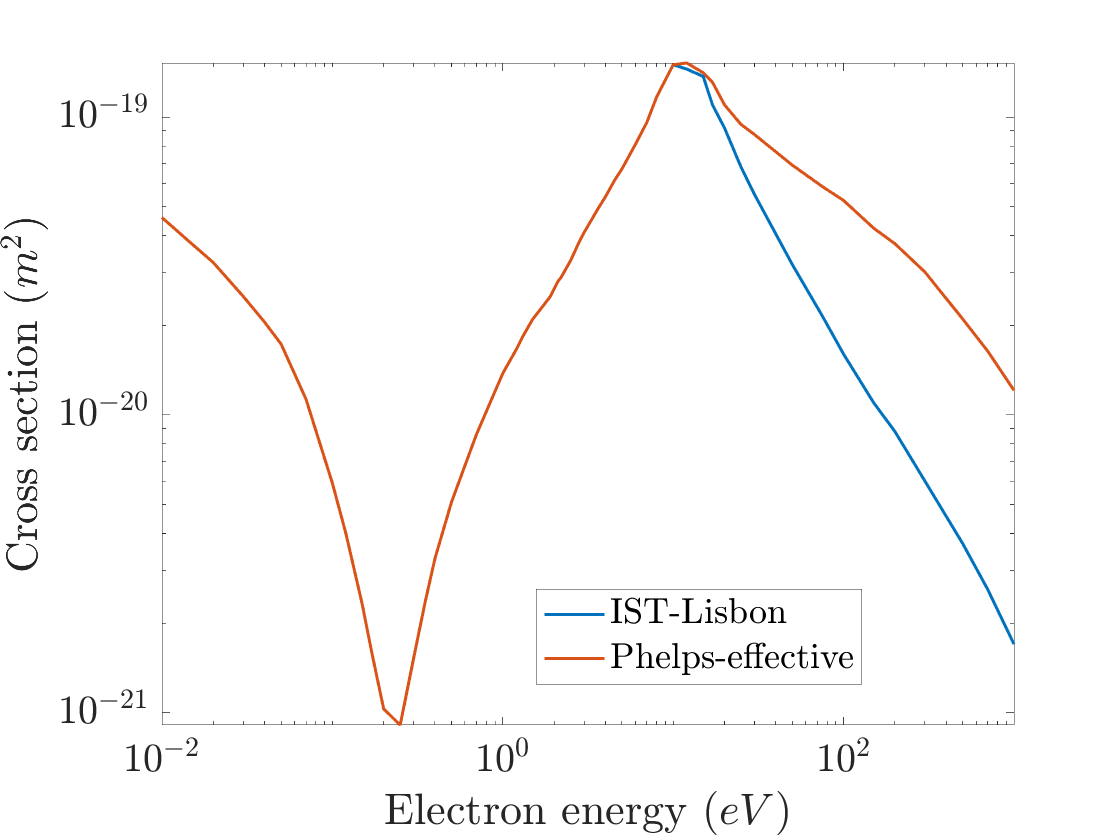
\includegraphics[width=0.6\textwidth]{./figures/ist-phelps}
\end{itemize}

\subsubsection{Phelps}
\begin{itemize}
\item Reference: \cite{Pitchford2013,Pitchford2017}
\item \cite{Pitchford2013}\\
The original version of the cross section set available at
LXCat was based on Frost and Phelps~\cite{Frost1964} as modified
in Tachibana and Phelps~\cite{Tachibana1981}.\\
\begin{itemize}
\item momentum transfer for $<4eV$: Milloy et al~\cite{Milloy1977}
\item momentum-transfer for $>8eV$: Fletcher and Burch~\cite{Fletcher1972}
\item total excitation cross section: Schaper and Scheibner~\cite{Schaper1969}
\item ionization cross section: Smith~\cite{Smith1930}
\end{itemize}
\item \cite{Pitchford2013}\\
The cross section set available at LXCat has been tested
through the comparison of calculated transport and reaction
rate coefficients with experiment in pure Ar for $1\le E/N \le 3000Td$.
Only the very early comparison with experiment in Frost and Phelps~\cite{Frost1964}
got published.
\item $O_2$ property measurement in $Ar-O_2$ mixture \cite{Tachibana1981}\\
Calculations using these cross section sets are found to yield electron attachment
coefficients in agreement with experiment to within experimental
uncertainty. Similarly, calculated electron drift velocities agree with measured values to within
$10\%$ for the $E/N$ range of our experiments.
\item The dataset is derived for use with the two-term
spherical harmonic expansion technique for solving the
electron Boltzmann equation.
\item Nakamura~\cite{Nakamura1988}, which similar to Biagi,
also used cross section of Milloy et al~\cite{Milloy1977}.
Figure below shows the similiarity of Biagi, Phelps to Milloy.\\
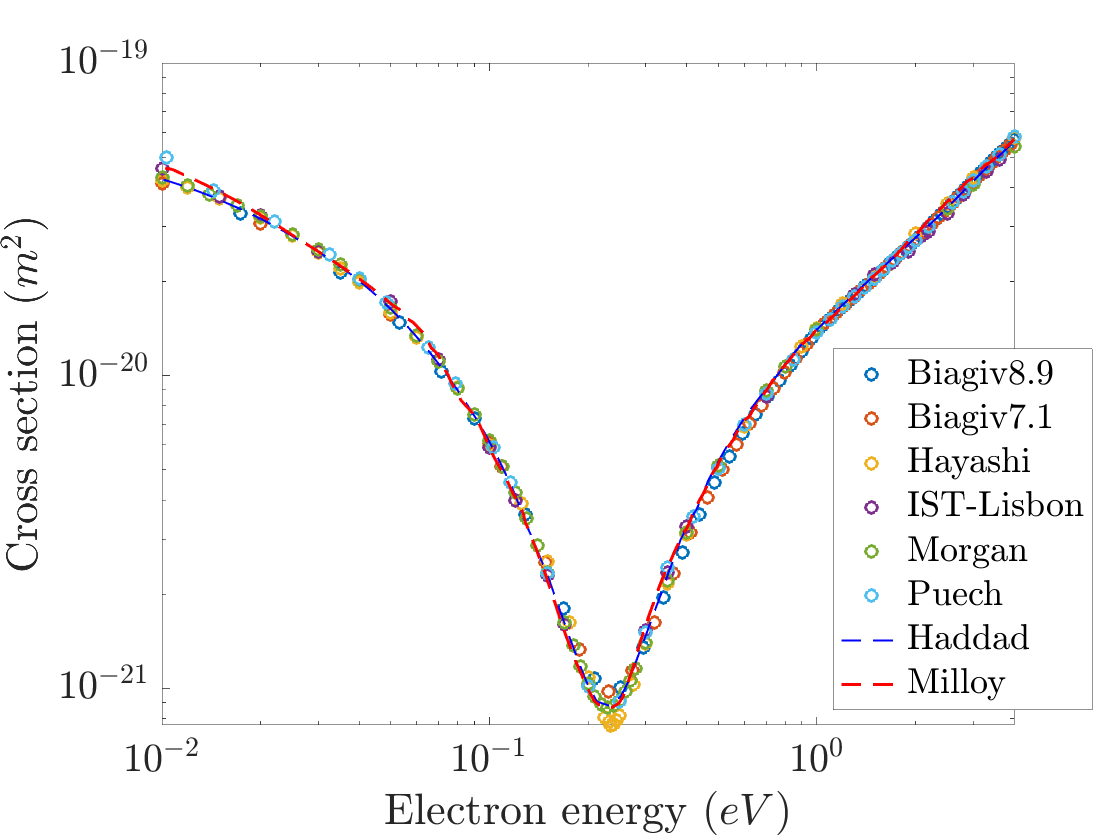
\includegraphics[width=0.6\textwidth]{./figures/milloy}
\end{itemize}

\subsubsection{Morgan}
\begin{itemize}
\item \cite{Pitchford2017}\\
For a wide variety of applications and starting in the mid-1970’s,
WL Morgan compiled the sets of electron scattering
cross sections in this database. $(\ldots)$
There is some overlap with datasets in the Phelps and Hayashi databases on LXCat
which is retained simply so that users can recover previously used data.
\item Not sure the sentence above corresponds to Ar.
Comparison with Phelps (IST-Lisbon) and Hayashi is shown below:\\
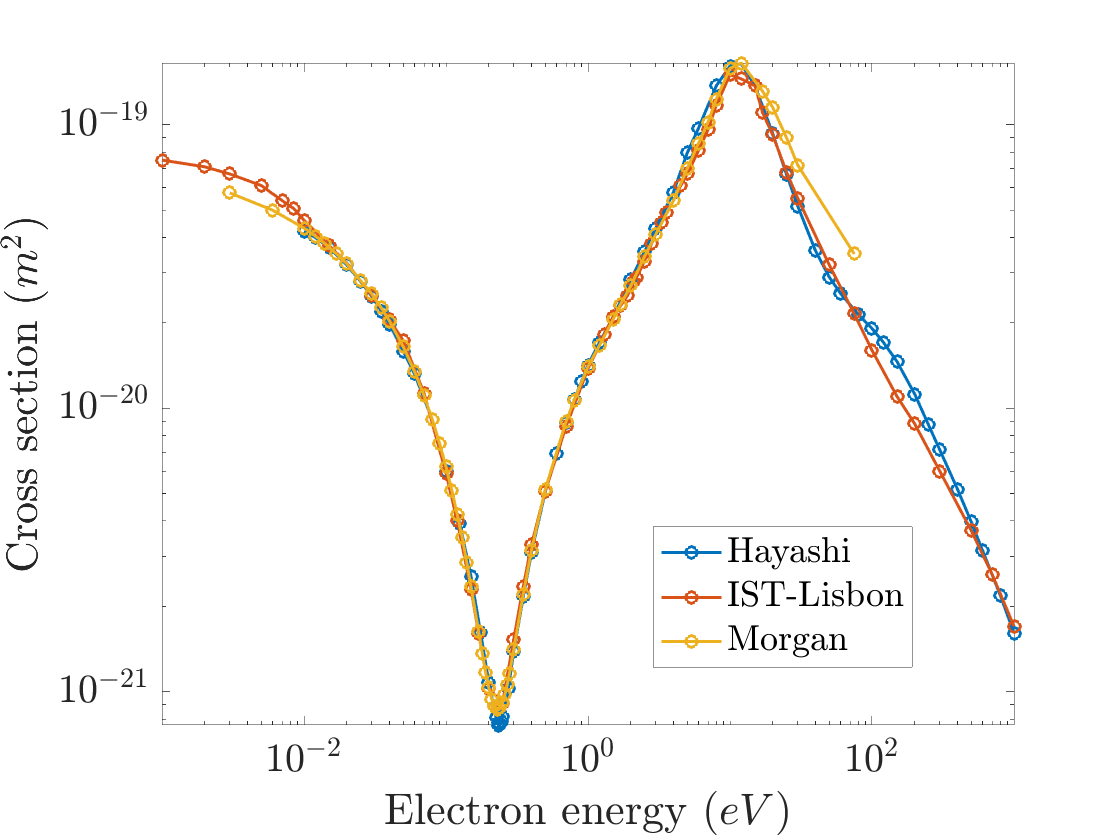
\includegraphics[width=0.6\textwidth]{./figures/morgan}
\item \cite{Pitchford2017}\\
One point to note is that the rotational excitation is
treated using a continuous approximation for rotation
(CAR) that is described by Frost and Phelps~\cite{Frost1962} and by
Morgan and Penetrante. The value of CAR is given in the
datasets but is not used in the on-line Boltzmann solver.
Thus, caution should be exercised in the interpretation of
the on-line calculations of swarm parameters at low $E/N$
where rotational excitation/deexcitation can have an
influence.
\item \cite{Pitchford2013}\\
The details of how Morgan’s data in noble gases were
compiled cannot be recalled at this point. However, the
procedure was standard: a choice was made about the level
of detail to be included for excitation (in this case, two
excited levels to represent allowed and forbidden transitions),
cross sections were estimated or guessed based on experiment
and theory, and then these cross sections were adjusted by
comparing measured swarm parameters with those calculated
using ELENDIF, Morgan’s two-term Boltzmann code (Morgan
and Penetrante 1990).
\item \cite{Pitchford2013}\\
The maximum energy in the data table or the elastic
momentum-transfer cross section in the Morgan database
is $75 eV$ and it is lower in the heavier noble gases. The
calculations reported here were done using the default
extrapolation scheme in BOLSIG+ assuming that cross
sections for energies higher than the last entry in the tables
decrease like $\log(\epsilon)/\epsilon$ where $\epsilon$ is electron energy, consistent
with the high-energy limit for cross sections for allowed
transitions in the Born approximation.
\end{itemize}

\subsubsection{Puech}
\begin{itemize}
\item Reference: \cite{Pitchford2013,Puech1986}
\item \cite{Pitchford2013}\\
The article by Puech and Torchin~\cite{Puech1986} describes in detail
the procedure used for the compilation and consistency
checking of this cross section set by comparisons with selected
experiments.
\item \cite{Puech1986}\\
we use an appropriate code which solves the Boltzmann equation in the usual two-term spherical
harmonic expansion.
\item \cite{Puech1986}\\
For elastic processes, we have used the momentum transfer cross section
given by Frost and Phelps~\cite{Frost1964} except in the range
$0.014-4eV$ where we have adopted the data of Milloy~\cite{Milloy1977}.
In LXCat databases, Puech seems to be interpolated between these two literatures.
For $<0.014eV$, data seems to be extrapolated.\\
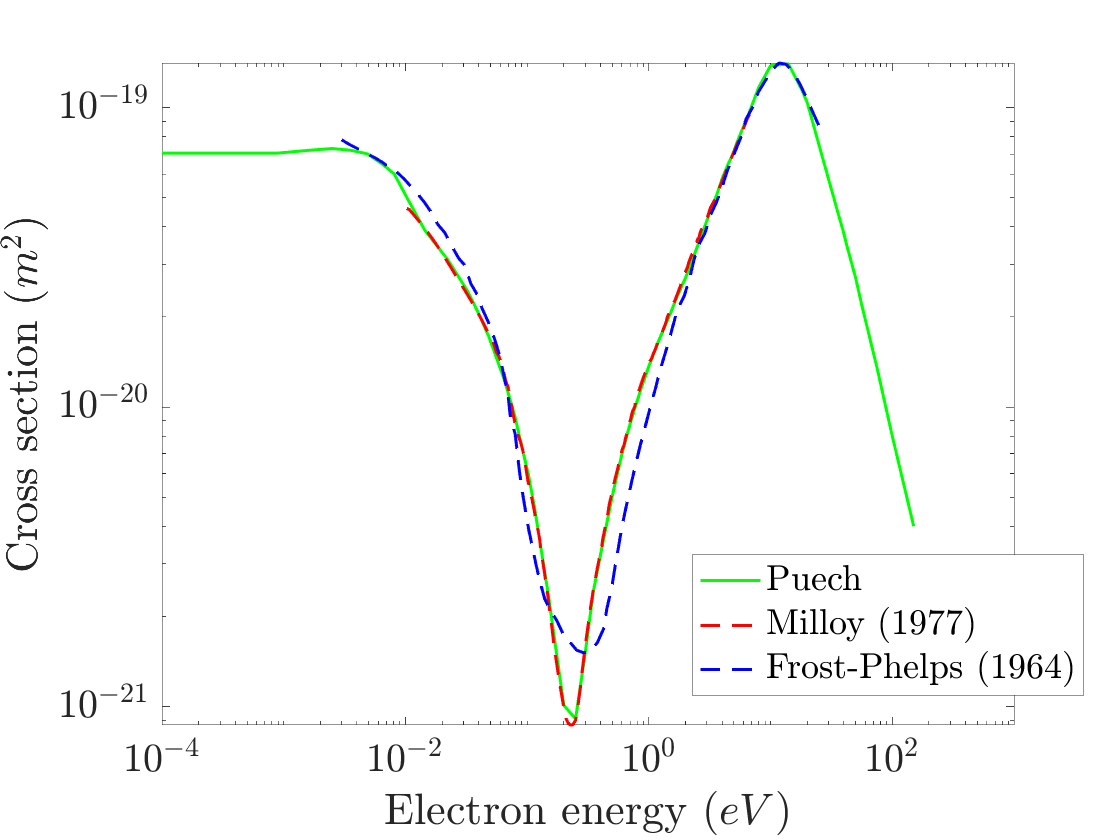
\includegraphics[width=0.6\textwidth]{./figures/puech}
\item Like other Boltzmann analysis, a set of cross sections are chosen from different literatures,
and compared the swarm parameters.
\item \cite{Pitchford2017}\\
Calculations of swarm parameters were made using a two-term Boltzmann
solver as well as the multiterm solver developed by
S\'{e}gur and Bordage~\cite{Segur1989}.
\end{itemize}

\bibliography{references.bib}

\end{document}